\documentclass{scrbook} % <= Druckversion: "scrbook" / Bildschirmversion: "scrreprt"
\usepackage[english,bibtex]{osm-thesis} % <= Sprache der Arbeit ("ngerman"/"english"), Biblatex-Backend ("bibtex"/"biber")
\usepackage{my-own-stuff}

% ABOUT
\newcommand{\thesistype}{Arbeit zur Erlangung des Grades \enquote{Master~of~Science} der Digital-Engineering-Fakultät der Universität~Potsdam}
\newcommand{\thesisauthor}{Vincent Opitz}

% Modelling carbon-aware scheduling

\newcommand{\thesistitle}{A Parameterizable Test Bed for Carbon Aware Job Scheduling}
\newcommand{\thesistitleother}{Ein parametrisierbares Testbed für kohlenstoffbewusste Jobplanung} % <= das Studienreferat verlangt einen deutschen UND englischen Titel

% LICENSE
\usepackage[type={CC},modifier={by-sa},version={4.0},lang=English]{doclicense}

% ADVISOR & REVIEWERS
\newcommand{\thesisadvisorlabel}{Betreuer:in}%
\newcommand{\thesisadvisor}{%
	Prof.\,Dr.\,rer.\,nat.\,habil.\,Andreas Polze\\
	Universität Potsdam,\\
	Digital Engineering-Fakultät, \\
	Fachgebiet für Betriebssysteme und Middleware}
\newcommand{\thesisreviewerlabel}{Gutachter:in}%
\newcommand{\thesisreviewers}{%
	Prof.\,Dr.\,Jack Alsohere\\
	University of San Serife\\
	Facultiy of Computer Doings%
	\and
	Amelia van der Beenherelong\\
	ACME Cooperation}

% IMPORTANT DATES
\newcommand{\thesishandindate}{\today}%
%\newcommand{\thesisdefensedate}{\formatdate{27}{9}{2004}}%

% PUBLICATION SERVER
%\newcommand{\thesisdoi}{https://doi.org/10.25932/publishup-49913}
%\newcommand{\thesisurn}{https://nbn-resolving.org/urn:nbn:de:kobv:517-opus4-499134}

% DOCUMENT
% run bibtex thesis if you change the bibliography file
% otherwise changes may not be compiled
\bibliography{bibliography}
\bibliography{web}

\begin{document}

	% Einband
	\pagenumbering{alph}
	\ifisbook\begin{titlepage}
	\setlength{\evensidemargin}{0.5\evensidemargin+0.5\oddsidemargin}
	\setlength{\oddsidemargin}{\evensidemargin}

	\centering

	\raisebox{-0.5\height}{
\includegraphics[width=5.5cm]{images/hpi_logo_black.pdf}}
	\hspace*{.2\textwidth}
	\raisebox{-0.5\height}{
\includegraphics[width=4cm]{images/uni_logo_black.pdf}}

	\vfill
	{\usekomafont{title}\thesistitle\par}\par
	\vspace*{\baselineskip}
	{\usekomafont{subtitle}\thesistitleother\par}\par
	\vspace*{\baselineskip}
	{\smallskip\usekomafont{author}\thesisauthor\par}\par

	\vfill\vfill
	{\usekomafont{date}\thesistype\par}\par

\end{titlepage}\fi
	\ifisbook\cleardoubleemptypage\fi

	% (Haupt-)Titelseite, Abstract, ggf. Danksagung & Inhaltsverzeichnis
	\pagenumbering{roman}
	\begin{titlepage}
	\setcounter{page}{1}
	\centering

	% TITLE PAGE

	\raisebox{-0.5\height}{
\includegraphics[width=5.5cm]{images/hpi_logo_srgb.pdf}}
	\hspace*{.2\textwidth}
	\raisebox{-0.5\height}{
\includegraphics[width=4cm]{images/uni_logo_srgb.pdf}}

	\vfill
	{\usekomafont{title}\thesistitle\par}\par
	\vspace*{\baselineskip}
	{\usekomafont{subtitle}\thesistitleother\par}\par
	\vspace*{\baselineskip}
	{\smallskip\usekomafont{author}\thesisauthor\par}\par

	\vfill\vfill
	{\usekomafont{date}\thesistype\par}\par

	\clearpage
	% BACK TITLE PAGE

	\begingroup
	\ifcsvoid{doclicenseThis}{\phantom{}}{%
		\begin{minipage}[t]{\textwidth}
			\noindent%
			\begin{flushleft}
				\small
				Unless otherwise indicated, this work is licensed under a \doclicenseLongType license:\\
				\doclicenseIcon\doclicenseLongNameRef.\\
				This does not apply to quoted content from other authors and works based on other permissions.\\
				To view a copy of this license, visit \url{\doclicenseURL}
			\end{flushleft}
		\end{minipage}}%
	\par\vfill
	\noindent
	\begin{otherlanguage}{ngerman}
	\begin{minipage}[b]{\textwidth}
		{\raggedright\small

		% author & title
		{\textbf{\sffamily{\thesistitle \\ (\thesistitleother)}}}\\
		von {\thesisauthor}
		\medbreak
		{\thesistype}
		\medbreak

		\ifcsvoid{thesisreviewers}%
		% advisor only
		{\def\\{ \tabularnewline & }%
		\edef\tempa{\thesisadvisor}%
		\begin{tabular}{@{}l@{\hspace*{1ex}}l@{}}
			{\textbf{\sffamily{\thesisadvisorlabel:}}} & \tempa
		\end{tabular}}
		% advisor + reviewers
		{\def\\{ \tabularnewline & }%
		\def\smalllinespace{\addlinespace[\smallskipamount]}%
		\def\and{ \tabularnewline \noexpand\smalllinespace & }%
		\edef\tempa{\thesisadvisor}%
		\edef\tempr{\thesisreviewers}%
		\begin{tabular}{@{}l@{\hspace*{1ex}}l@{}}
			{\textbf{\sffamily{\thesisadvisorlabel:}}}  & \tempa \\\smalllinespace
			{\textbf{\sffamily{\thesisreviewerlabel:}}} & \tempr
		\end{tabular}}
		\medbreak

		\ifcsvoid{thesishandindate}%
		{} % no hand in, no defense
		{\ifcsvoid{thesisdefensedate}%
			% hand in only
			{\begin{tabular}{@{}l@{\hspace*{1ex}}l@{}}
					{\textbf{\sffamily{Datum der Einreichung:}}} & {\thesishandindate}
				\end{tabular}}%
			% hand in + defense
			{\begin{tabular}{@{}l@{\hspace*{1ex}}l@{}}
					{\textbf{\sffamily{Datum der Einreichung:}}} & {\thesishandindate}  \\
					{\textbf{\sffamily{Datum der Disputation:}}} & {\thesisdefensedate}
				\end{tabular}}}
		\medbreak
		}%
		{\ifcsvoid{thesisdoi}%
		{}% not published
		{
			\vspace*{4\baselineskip}%
			\raggedright\small\noindent
			\iflanguage{ngerman}{Online veröffentlicht auf dem Publikationsserver der Universität Potsdam}{Published online on the Publication Server of the University of Potsdam}:\\
			\url{\thesisdoi}\\
			\url{\thesisurn}%
		}
		}%

	\end{minipage}
	\end{otherlanguage}
	\endgroup

\end{titlepage}
	\ifisbook\cleardoubleemptypage\fi% => Wenn die Arbeit auf Deutsch verfasst wurde, verlangt das Studienreferat KEINEN englischen Abstract

% % englischer Abstract
%\null\vfil
%\begin{otherlanguage}{english}
%\begin{center}\textsf{\textbf{\abstractname}}\end{center}
%
%\noindent Lorem ipsum dolor sit amet, consetetur sadipscing elitr, sed diam nonumy eirmod tempor invidunt ut labore et dolore magna aliquyam erat, sed diam voluptua. At vero eos et accusam et justo duo dolores et ea rebum. Stet clita kasd gubergren, no sea takimata sanctus est Lorem ipsum dolor sit amet. Lorem ipsum dolor sit amet, consetetur sadipscing elitr, sed diam nonumy eirmod tempor invidunt ut labore et dolore magna aliquyam erat, sed diam voluptua. At vero eos et accusam et justo duo dolores et ea rebum. Stet clita kasd gubergren, no sea takimata sanctus est Lorem ipsum dolor sit amet.
%
%\end{otherlanguage}
%\vfil\null


% => Wenn die Arbeit auf Englisch verfasst wurde, verlangt das Studienreferat einen englischen UND deutschen Abstract (der dt. Abstract kann dann ggf. auch ans Ende der Arbeit)

% deutsche Zusammenfassung
\null\vfil
\begin{otherlanguage}{ngerman}
\begin{center}\textsf{\textbf{\abstractname}}\end{center}

\noindent 

\todo summarize thesis

Lorem ipsum dolor sit amet, consectetur adipiscing elit, sed do eiusmod tempor incididunt ut labore et dolore magna aliqua. Ut enim ad minim veniam, quis nostrud exercitation ullamco laboris nisi ut aliquip ex ea commodo consequat. Duis aute irure dolor in reprehenderit in voluptate velit esse cillum dolore eu fugiat nulla pariatur. Excepteur sint occaecat cupidatat non proident, sunt in culpa qui officia deserunt mollit anim id est laborum.

%- temporal shifting
%- include the costs of pausing a job (saving work and resuming it)
%- include costs of shutting down or starting additional compute nodes
%- include frequency scaling 
%- provide a model for simulating scheduling of jobs, and also model what information need to provide to increase CO2 efficiency. 

%C The study aims to [state the objectives or goals of the research]. Through [methodology/approach], %data was collected from [source or population]. The findings reveal [main results or discoveries].

%The analysis highlights [key insights or implications], shedding light on [broader significance or relevance]. This research contributes to the understanding of [specific field or subject area], offering [potential applications or recommendations].

%Overall, this thesis provides valuable insights into [topic] and offers avenues for further exploration in [related areas].

\end{otherlanguage}
\vfil\null




	%\ifisbook\cleardoubleemptypage\fi\vspace*{\fill}
\begin{center}\textsf{\textbf{Danksagung}}\end{center}

\noindent Lorem ipsum dolor sit amet, consetetur sadipscing elitr, sed diam nonumy eirmod tempor invidunt ut labore et dolore magna aliquyam erat, sed diam voluptua. At vero eos et accusam et justo duo dolores et ea rebum.

\vspace*{\fill}
	\tableofcontents
	\cleardoublepage

	% Textteil
	\pagenumbering{arabic}

	\chapter{Introduction and Motivation}

In times of climate change, the need to reduce carbon emissions is prevalent. 
One area of interest is carbon produced via electrical power used in data centers. 
However, not all power is produced equally: while a data center may source its power from the public grid, the public grid itself is sourced from different producers. 
These include high-carbon intensive technologies such as coal and gas but also include low-carbon sources such as solar and wind. 
The latter, renewables and especially solar, follow a diurnal rhythm over the day as shown in Figure \ref{fig:energy_mix}.

\begin{figure}
    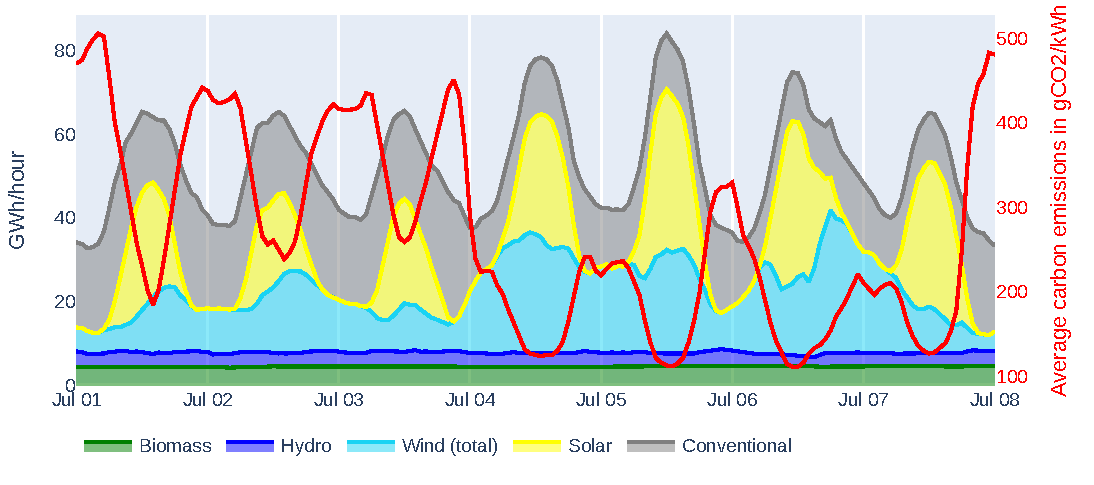
\includegraphics[width=\linewidth]{agorameter/energy_production_week.pdf}
    \caption[short]{Mix of energy production in Germany for the first week of July 2024 with the resulting hourly average carbon emissions per kWh\webcite{web_agora}. Solar production peaks at noon, reducing carbon intensity, creating times, where jobs may be scheduled more carbon efficiently.}
    \label{fig:energy_mix}
\end{figure}

As the sun shines more during the day, a bigger part of the total power production then comes from solar, reducing the overall carbon intensity of the grid.
This can be used for \emph{carbon-aware scheduling}, by planning work in data centers to be executed during such low-intensity times, the overall carbon can be reduced.

Data centers are currently projected to experience exponential growth in their power requirements, largely fueled by pushes in AI.\cite{schwartz_green_2019}

Current work on carbon-aware scheduling includes shifting jobs temporally and spatially. 
One common theme among them, however, is that the workload models do not include program heterogeneity: while real-world programs may include high-powered times for computation and low-powered times e.g. I/O, this is not reflected in literature. 
Another common strategy for executing jobs during low-carbon timeframes is to \emph{suspend \& resume}: a job may be, for example, stopped as carbon intensity is increasing and resumed when a certain threshold is reached. 
This generally assumes, that resuming a job carries no overhead. 

In this work, we will improve upon the homogeneous, no-overhead workload model used in literature, by measuring an AI program and deferring a new model upon that.

The research question will be the following:

\begin{enumerate}
    \item Are there carbon savings under a workload model including resume-overhead and power-heterogeneity?
    \item How does this compare to previous work in the field using the homogeneous model?
    \item Which jobs are better suited for carbon-aware scheduling?
\end{enumerate}

	
	\chapter{Background}
\label{chap:backgroud}

In this chapter, we will introduce some basic terminology as well as provide further information surrounding carbon scheduling.

\section{The Composition of the Public Grid}

As outlined in the previous chapter, the energy production of the public grid is supplied by different producers.
Renewables create order of magnitudes less emissions than conventional technologies.  

\begin{table}[h!]
    \centering
    \begin{tabular}{|c|c|}
    \hline
        Technology & gCO\textsubscript{2}/kWh \\ \hline
        Nuclear & 5 \\ \hline
        Hydro, Wind & 12 \\ \hline
        Solar & 35 \\ \hline
        Gas & 530 \\ \hline
        Coal & 1079 \\ \hline
    \end{tabular}
    \caption{The carbon intensity of different energy sources.\webcite{web_electricitymaps}}
    \label{tab:carbon_intensities}
\end{table}

As supply and demand in power need to be balanced, the composition of the grid changes according to changes in demand.
On the day-scale, there are atleast two dimensions to this. For once, there is the aforementioned diurnal rhythm of solar production.

\todo[inline]{This needs some better wording, did not get to this yet.}
\todo[inline]{I also wanted to mention the duck curve, or how there are changes to demand from human patterns.}

In addition to that, there is also a seasonal effect on the energy grid composition:
As shown in Figure \ref{fig:energy_mix_year}, during warm seasons (e.g. July), more solar is produced than in colder seasons, and the share in renewables rises accordingly.

\begin{figure}
    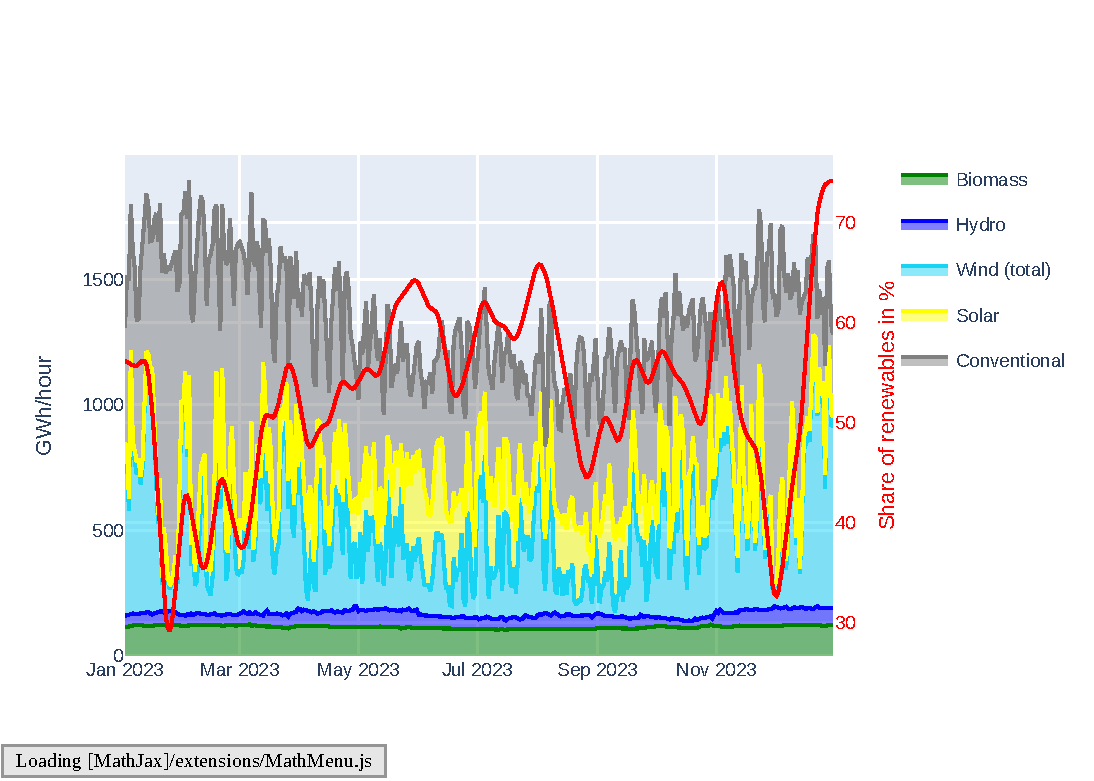
\includegraphics[width=\linewidth]{agorameter/energy_production_year.pdf}
    \caption[short]{Mix of energy production in Germany in 2023 \webcite{web_agora}. Seasonally, renewables will be highest during summer but may also spike during holidays. Thus, yearly time scopes can also be considered for carbon aware scheduling.}
    \label{fig:energy_mix_year}
\end{figure}

The demand for power also has an effect on the overall composition. 
During times of low demand, less conventional power needs to be produced and renewables have a higher share as well.
This can be seen in the seasonal Figure: during Christmas holidays in December, people spend more time at home, requiring less additional conventional energy (e.g. for industrial consumers, as people also work less).

All the above is a local or national view on the public grid. 
When looking at energy production globally, a spatial dimension is added. 
This takes effect in the form of different countries having peak solar production at different times (following the earth's rotation), but also takes effect in the composition of production capabilities.
Some countries may have less investment in renewables or may use nuclear power plants, which are also deemed low-carbon\todo{Needs citation} but have less of a seasonal or diurnal rhythm (if they are not limited by lack of cooling water \webcite{noauthor_heatwave_2023}).

Thus, national public grids have a certain affinity for carbon aware scheduling\cite{wiesner_lets_2021}. Generally, the higher the solar capacities, the higher the potential carbon saving from such an approach. 

\section{Power Grid Signals}
Carbon-aware scheduling commonly uses one of two possible metrics or signals: the \emph{average emissions} are the metric describing the amount of carbon per unit of energy. These are calculated using the weighted average of all power supplies at a point in time.

Another metric is the \emph{marginal emissions}, answering the question of "if more energy is used at this point in time, how much carbon does that cost?".
\todo[inline]{Make a idealized graph on how the marginal emissions work}

The marginal emissions are closely related to the way energy producers in- or decrease production.
In order to reduce electricity prices, additional demand on the grid is dispatched to the cheapest power plant with remaining capacity. 
These power plants, also called \emph{marginal power plants}, have a correlation to the carbon emissions.
With the cheapest power coming from renewables, additional demand is supplied with more expensive, more carbon intensive, conventional power plants.

Two providers of signal data are \emph{Electricitymaps}\webcite{web_electricitymaps} and \emph{WattTime}\webcite{web_watttime}.
Electricitymaps has a free access API for historical and current average emissions. Both providers only offer the marginal signal commercially, however. 

Going further, the average signal will be used. 
Note should be taken that current literature is still split on which signal is best. 
A recently released and aptly named paper by Sukprasert et. al \cite{sukprasert_limitations_2024} may be read for further information on grid signals, as well as arguments for either signal.

Out of these, reasons for using the average signal is, for example, \emph{curtailment}. 
Curtailment encompasses any methods that reduce the amount of produced renewable energy. As the power grid always needs to have a balance between demand and production, curtailment methods such as turning of wind turbines, selling power at a loss, or charging batteries may be used. 
Carbon aware scheduling via the average emissions signal lowers the amount of curtailment needed, as demand for energy would increase at those times.
Another argument made, for example by Fridgen et al. \cite{fridgen_not_2021}, is that by increasing power demand during times when renewable production is high, investments in renewables would be promoted. 
Lastly, as renewable energy is generally cheaper in production than non-renewable energy\todo{Need a citation here!}, scheduling work on low carbon-periods coincides with cheaper energy prices as well. While this would not reduce costs on most energy contracts, there are also some contracts that use dynamic pricing \footnote{One example for dynamic pricing is \emph{Tibber}\webcite{web_tibber}}

\paragraph{Workloads in a Datacenter} According to Tanenbaum and Woodhull\cite{tanenbaum_operating_2006}, there are three environments in which scheduling may take place. \emph{Batch systems} describe environments in which there is no user interaction. 
Scientific simulations and computations, machine learning workloads, and data processing tasks are examples of these workloads\cite{sukprasert_limitations_2024}.
A user may submit their job, and it would be executed according to the scheduler at some point in time. 
On the contrary, in \emph{interactive} settings, a user interacts with the system, and thus expects quick responses to their inputs. An example of an interactive job are web requests, which should be answered quickly inherently.
The last environment are \emph{real time} systems. There, deadlines and predictability dictate how a scheduler operate.

For this work's topic, (temporal) carbon-aware scheduling, only batch systems will be looked at as they allow more freedom to the times of scheduled jobs.

\section{Measuring Power}

There are multiple options for measuring the power of a given computer. One way of classifying these options is categorizing them under \emph{logical measurements} or \emph{physical measurements}.

Logical ones create a model on some metrics and derive the used power. One example is using Linux' \emph{perf} tool to read hardware performance counters, then assigning an energy cost to select counters and multiplying that. 

Advantages of choosing a logical approach are that no external hardware is needed and that the overhead of the measurement is low, as the hardware counters are being kept track of anyway. 
Disadvantages on the other hand are that such a model has to be created or chosen and includes some form of error as all models do.

Physical measurements follow another route; measurement devices are put between the operating hardware and the power supply. 
The point where a power measuring device is inserted dictates what could and could not be measured, a wall mounted measurement device could only measure all power going into a computer and not differentiate between individual programs.

Advantages of physical measurements are that they can give a more holistic measurement of a system as would be the case for a wall mounted measurement device. 
Portability is an issue however, unlike operating-system supported tools such as perf, a measurement device needs more effort to be used on another system (or be entirely not useable, for example when such devices are only rated for a certain power level).

% \paragraph{Power Consumption of a Computer}
% As there will be power measurements in \ref{sec:power_measurements}, some basic understanding of energy and power used for computation will be provided:
% \begin{itemize}
%     \item I could mostly borrow from the EBRH slides; there is some base power needed that is correlated to the hardware (dynamic and static energy)
%     \item this also depends on frequency (which is why later we set our CPU frequency to some hard coded value [or do not do that in the case of my GPU lol])
%     \item basically, use this paragraph to outline all things we take care of in my power measurements
% \end{itemize}
	\chapter{Related Work}

- generell die literaturrecherhe mal auswerten aus dem google docs, perhaps da auch ein paar statistics drauß machen. Wie sehr ist das Thema in der Literatur vertreten? 
lets wait a while
going green for less
greenslot
The War of the Efficiencies: the Tension between Carbon and Energy Optimization
	
	\chapter{Defining a New Workload model}

In order to improve on the homogenous, no startup-cost, workload model used in related work, we will first conduct power measurements on a sample program, and then use that information for the new model.

\section{Power Measurements on Machine Learning Jobs}
\label{sec:power_measurements}

\paragraph{The test environment}

The experiments were run on my personal computer, the components of that are listed via the \emph{hwlist} tool, with some columns and rows being redacted for brevity:

The experiments are run on a personal computer, its specification being outlined in Table \ref{tab:measurement_environment}, the values being determined with Linux' \verb|hwlist| and \verb|lshw| tools.

\begin{table}[h!]
    \centering
    \begin{tabular}{|c|c|}
    \hline
        Operating system & Ubuntu 24.04 LTS \\ \hline
        Kernel & Linux 6.8.0-39-generic \\ \hline
        CPU & AMD Ryzen 5 1600X Six-Core Processor \\ \hline
        Memory & 16GiB \\ \hline
        GPU & GeForce GTX 1070 \\ \hline
    \end{tabular}
    \caption{Environment parameters of the power measurements}
\label{tab:measurement_environment}
\end{table}

\paragraph{Measurement tool}

Like outlined in Chapter \ref{chap:backgroud}, multiple measurement options exists. 
As the HPI has the \emph{Microchip MCP39F511N Power Monitor (henceforth called MCP)} on-site, they will be used as a physical measurement device.
The MCP is placed between the device to test and the wall mounted power supply. A picture of it can be found in figure \ref{fig:mcp}. It can report the current power consumption in 10 mW steps, each 5ms.

\begin{figure}
    \missingfigure{A figure of the MCP, ask Sven about this}
    \caption[short]{The MCP}
    \label{fig:mcp}
\end{figure}

\todo{I could include an extra paragraph on why the MCP is cool, and what it does differently, perhaps. Was there anything cool? I vaguely remember some measurement devices having two capacitors to more accurately determine usage}

The software used for reading out MCP data is \emph{pinpoint}\cite{kohler_pinpoint_2020}.

\paragraph{Measured Program}

Machine learning (ML) was used as the main motivation for suspend \& resume scheduling in the related works\cite {wiesner_lets_2021} and thus was also chosen by me to be measured and modeled. 

The concrete model and framework is secondary for our measurement. In our case, a small model\webcite{web_distilbertdistilroberta-base_2024} is chosen in order to have fewer data points for processing, as well as faster iterations on the measurement script. 

There is a vast amount of machine learning frameworks. 
For a high-level model, the feature set of the framework only needed to support checkpointing, resuming, and some basic form of logging. 
A glance at the documentation of popular frameworks such as \emph{torch}, \emph{tensorflow}, and \emph{huggingface} shows that these features are commonly supported. 

With not much bias towards any framework, huggingface was chosen.
The huggingface trainer supports callbacks, we modified a given ML script to also log timestamped events when a training iteration, for example, starts or ends. 
These events are then saved into another \verb|.csv| file for each experiment.

\paragraph{Conducted Experiments}

A script \verb|measure_roberta.sh| was used to execute each experiment. 
On a high-level view, the following experiments were conducted: 

\begin{enumerate}
    \item \label{experiment:full}Run the whole program start to finish
    \item \label{experiment:partial_checkpointed}Run it partially, checkpointing after some step, sleeping, resuming from that step
    \item \label{experiment:partial_checkpointed_aborted}Run it partially, checkpointing after some step but aborting before the next checkpoint. Then resume as above.
    \item \label{experiment:startup_only}Run only the startup phase up until the ML would start
    \item \label{experiment:baseline}Do nothing, measure the system at rest
\end{enumerate}

Experiment \ref{experiment:full} gives a baseline for what the job looks like without suspend \& resume. Number \ref{experiment:partial_checkpointed} and \ref{experiment:partial_checkpointed_aborted} would be used to determine the overhead of checkpointing the job. \ref{experiment:startup_only} would be used to validate the other ones. The last experiment is necessary to determine the baseline energy consumption of the environment.

To execute these experiments inside a repeatable bash script, additional command line parameters were added to the program. 
For example, a boolean parameter \verb|--resume_from_checkpoint| and an integer parameter \verb|--stop_after_epoch| are used for experiment \ref{experiment:full} to \ref{experiment:partial_checkpointed}. 
The way of conducting experiment \ref{experiment:startup_only} was to copy the script, and delete everything after the imports.

\paragraph{Creating repeatable measurements}

As this is being run on standard hardware on a standard operating system, all experiment are subject to noise. 
For example, \emph{Dynamic frequency and voltage scaling (DFVS)}, the OS technique of increasing CPU "speeds" according to work load add power in an uncontrolled way. Also, background tasks may happen \emph{randomly}, increasing power usage. 

Thus, for the testing, any foreground apps are closed. We also used the Linux tool \verb|cpupower|, as shown in snippet below, to set the CPU frequency to a set value of 3.6 GHz, which is the maximum frequency:

\begin{minipage}{\linewidth}
\begin{lstlisting}[language=bash, frame=single, numbers=none, caption={Used operating system information}, basicstyle=\ttfamily]
    MINFREQ=$(cpupower frequency-info --hwlimits | sed -n '1d;p' \
        | awk '{print $1}')
    MAXFREQ=$(cpupower frequency-info --hwlimits | sed -n '1d;p' \
        | awk '{print $1}')
    
    cpupower frequency-set --min ${MAXFREQ} &>/dev/null
    cpupower frequency-set --max ${MAXFREQ} &>/dev/null

    # ... conduct experiments

    cpupower frequency-set --min ${MINFREQ} &>/dev/null
    cpupower frequency-set --max ${MAXFREQ} &>/dev/null
\end{lstlisting}
\label{listing:setting_cpu_frequency}
\end{minipage}

As machine learning makes use of available GPUs, the frequency should also be similarly set to a defined value. 
NVIDIA provides guide on how to do so\footnote{\url{developer.nvidia.com/blog/advanced-api-performance-setstablepowerstate}}.
Our used GPU, the NVIDIA GTX 1070, is not capable of fixing the frequency as of the time of conducting these experiments. 
While it is supposed to be possible, there seems to currently be drivers issue preventing this\webcite{web_powerlimitissue}.
Thus, the frequency of the GPU was not fixed. 
To reduce the effect of frequency scaling here, the time between experiments was increased generously so that any impact from such scaling reoccurs throughout each run, reducing dependencies between runs.

During the training, data is downloaded and saved, which is however deleted before the next experiment. 
The python process is also not kept between runs, forcing a uniform load of any libraries.

\paragraph{Conducting each experiment}

Each experiment was re-run 10 times. Between each run, there is a \verb|sleep| period of 10 seconds and one of two minutes in the partial executions. 
Additionally, \verb|pinpoint|'s feature of measuring before and after the actual program-to-test would be used. 
This leads to a period of 30 seconds being measured around the program execution. 
Plotting these additional time frames gives a quick visual indicator whether experiments are sufficiently isolated from each other, ergo when the power draw is at the baseline as the actual program starts.

As there is some data being downloaded and persisted during the execution of the ML, before each run, that data is removed,

\paragraph{Collected data}

For each experiment, a named and timestamped folder is created in the \verb|/power-measurements| folder of my repository. Each folder then holds a \verb|.csv| with pinpoint's timestamped power measurements. 
The added timestamped-logging is saved into another \verb|.csv|. 
On the way to the final measurements, we plot each experiment early and visually spot if there are any obvious errors or mistakes.

\paragraph{Determining the baseline power draw}

Beginning with the most exiting experiment, determining the baseline and testing the amount of the underlying environment. 
One sample run is shown in Figure \ref{fig:plot_baseline}.
The blue dots in figure represent each data point. The red line is a smoothed Gaussian trend line with $\sigma = 2$. 
Dark-green vertical lines are the logged or derived "events" for each run. In this case, nothing happens, so it is only the start and end of \verb|sleep 120|. 
Notice how the trace starts 30 seconds before the start and continues for another 30 seconds because of the aforementioned \verb|pinpoint| feature.
Going further, these additional measurements will be redacted for brevity.

\begin{figure}
    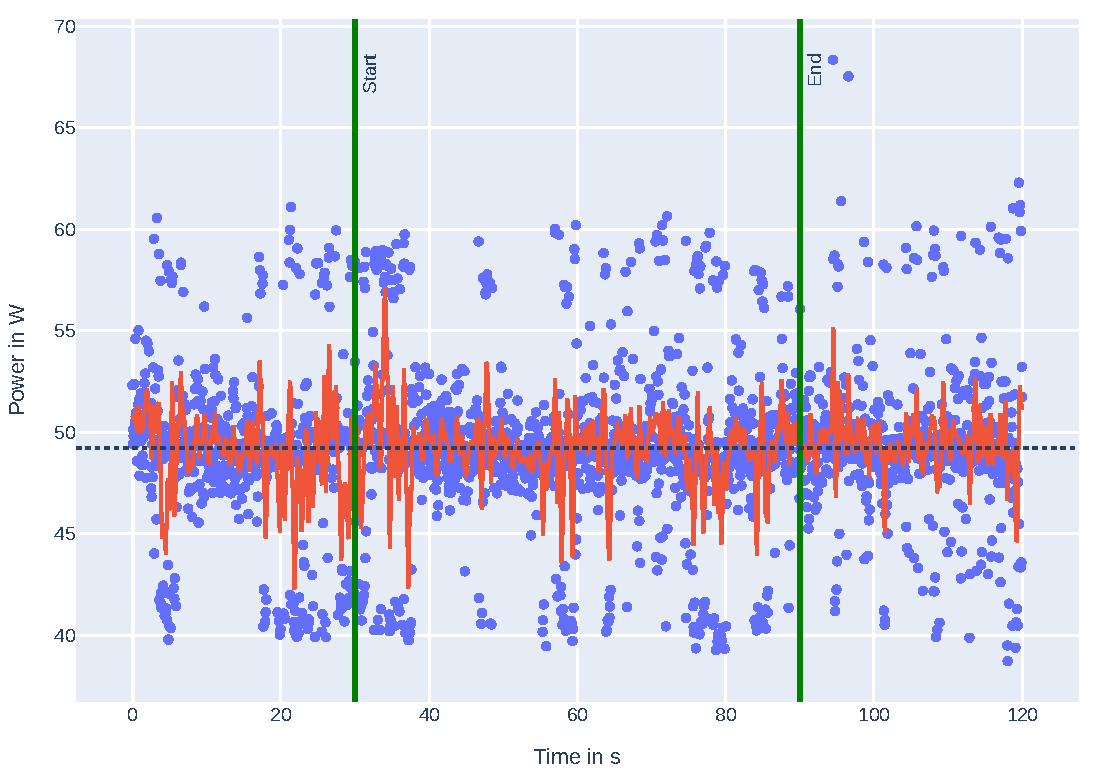
\includegraphics[width=\linewidth]{power-measurements/measurements_sleep_0714004033/plot.pdf}
    \caption{Sample run of the baseline experiment. The dotted line is the global average. The red line is a smoothed Gaussian trend line.}
    \label{fig:plot_baseline}
\end{figure}

Across all 10 runs, the average baseline power draw is calculated via the mean of all data points. This comes out as an average of 49.8 W with a standard deviation of 4.4 W.

The baseline power draw will be less interesting going further, but will put perspective on the power draws of the other experiments. The standard deviation should give a broad idea of how much noise is in the system environment.

\paragraph{The non-interrupted run}

For the non-interrupted machine learning run, a sample run is provided in Figure \ref{fig:plot_full}. 
Figure \ref{fig:plot_full_stacked} shows the stacked trend lines of the 10 different runs.
For simplicity's sake, we refrained from doing more elaborate statistical analysis on the different runs as the visual check of them being very similar seemed enough.

\begin{figure}
    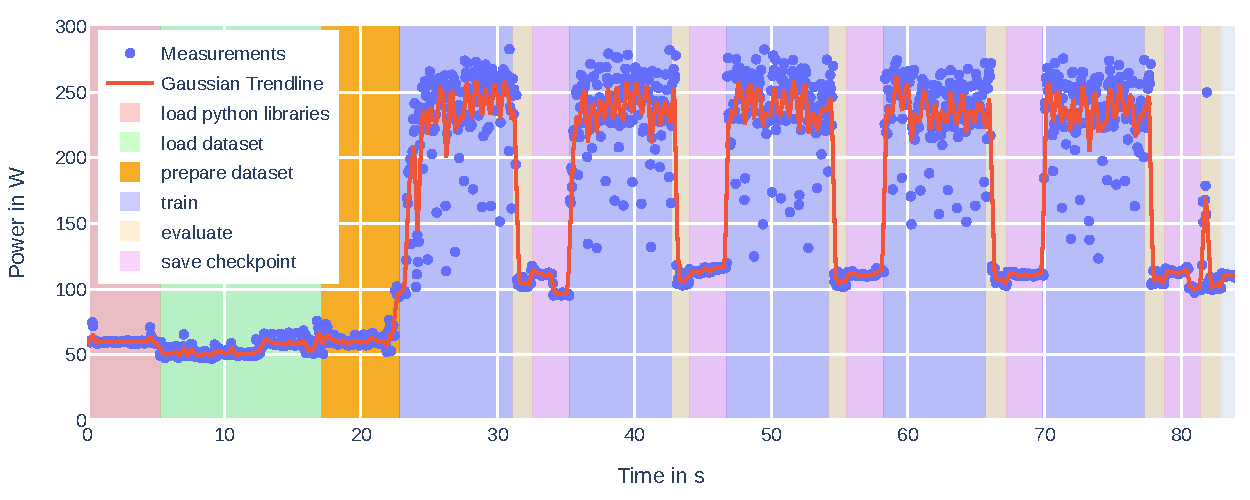
\includegraphics[width=\linewidth]{power-measurements/measurements_roberta_full_0714010405/plot.pdf}
    \caption{Sample run of the full run experiment, the background indicates the phase as determined by the added logging}
    \label{fig:plot_full}
\end{figure}

\begin{figure}
    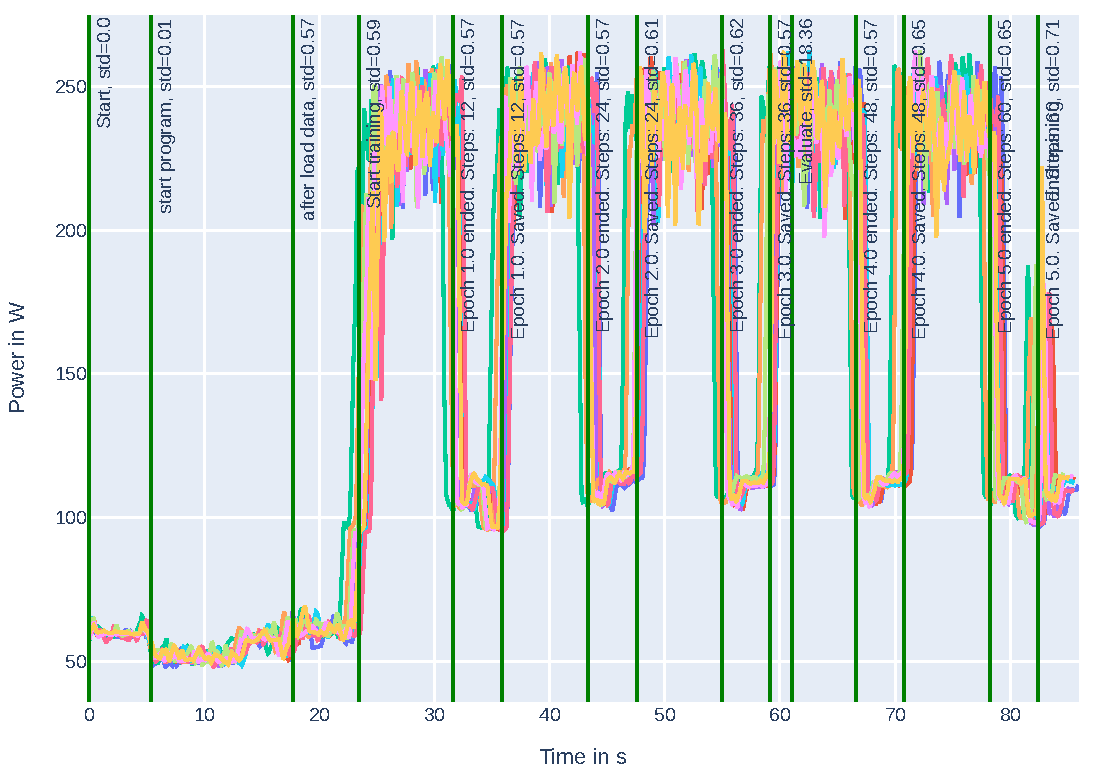
\includegraphics[width=\linewidth]{power-measurements/stacked_plots/roberta_full_0714.pdf}
    \caption{All full-run trend lines stacked. }
    \label{fig:plot_full_stacked}
\end{figure}

The main takeaways from these measurements are:

\begin{enumerate}
    \item There is a long (about 25\%) start-up phase, which is spent in starting python, loading libraries, and loading data to disc.
    \item There are periodical work-phases; a high-power training phase would be followed by low-power evaluation\todo{Uhm, where did my evaluation phase markers go?? They are mushed together as they share a label} phase and a low-power checkpointing.
    \item A higher variance in measurements occurs during the training phases in comparison to the others.
\end{enumerate}

This already shows, that improvements upon the constant-power model used in \cite{wiesner_lets_2021} are possible. 
For example, in this case the start-up phase has a much lower power-draw than the work-phase.

\paragraph{Results of the checkpoint and restore experiment}

Similarly to before, results will be discussed using the stacked plots \ref{fig:plot_partial_saved_stacked} and \ref{fig:plot_partial_saved_continue_stacked}; each individual run is plotted in the repository, however.

\begin{figure}
    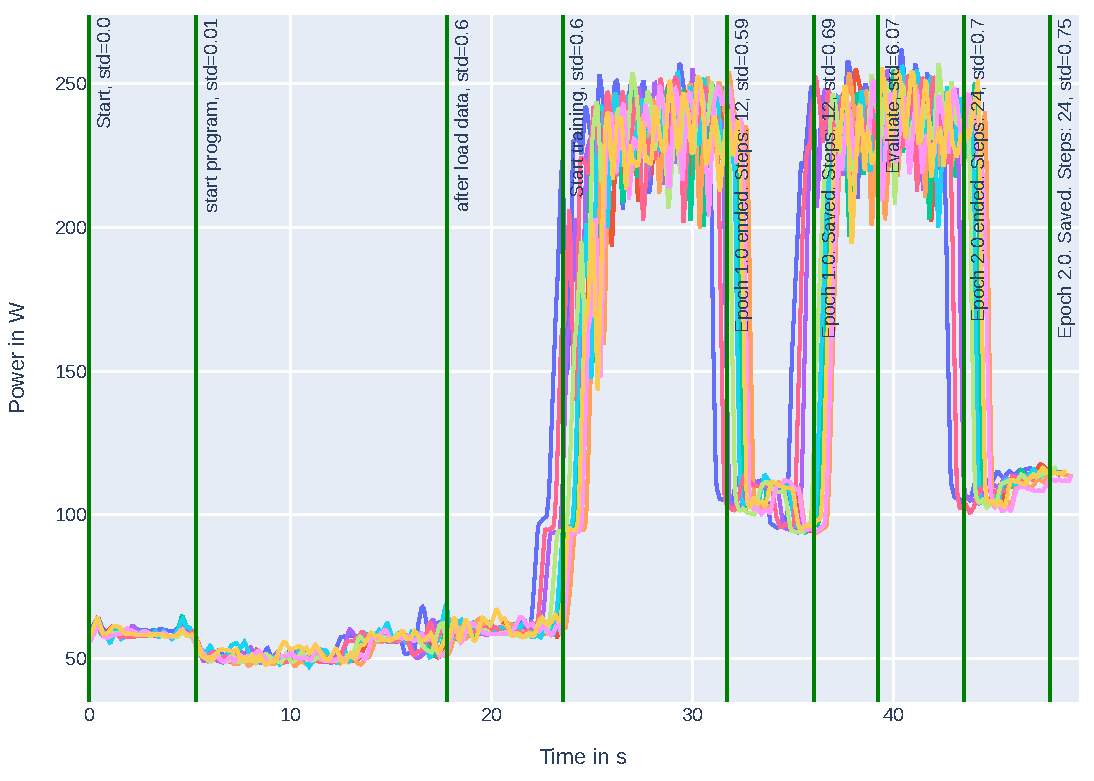
\includegraphics[width=\linewidth]{power-measurements/stacked_plots/roberta_stop_after_saving.pdf}
    \caption{Stacked trend lines of the experiment for stopping after the second epoch}
    \label{fig:plot_partial_saved_stacked}
\end{figure}

\begin{figure}
    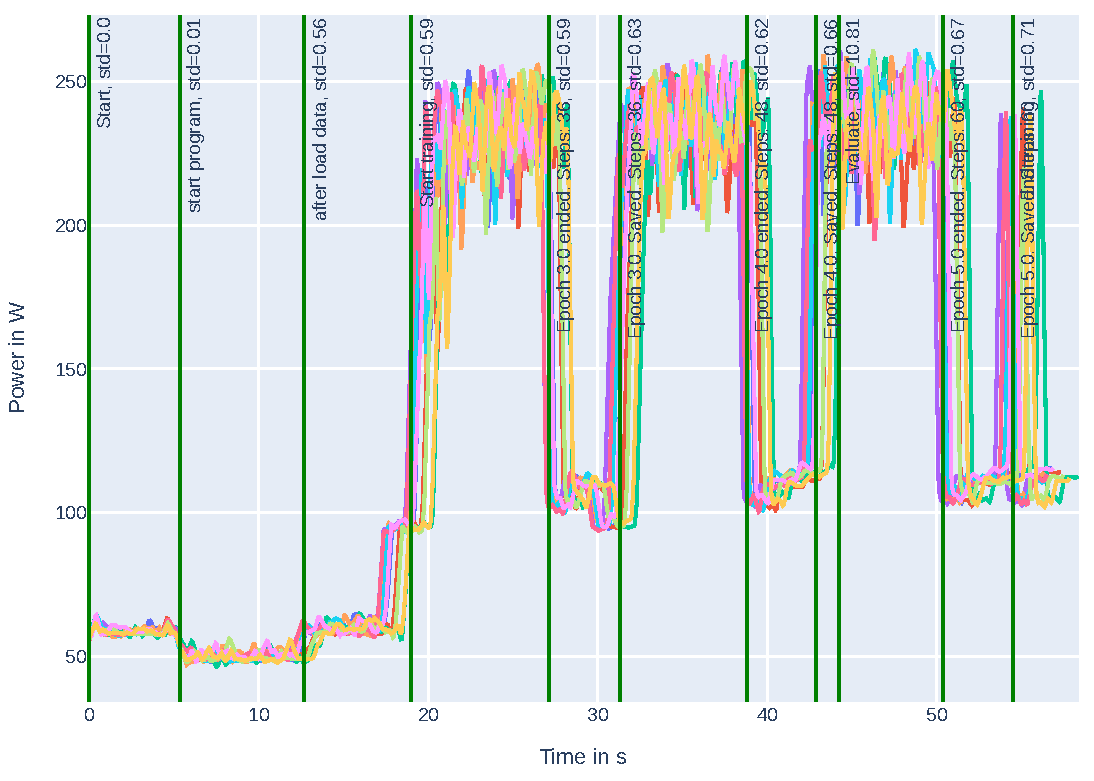
\includegraphics[width=\linewidth]{power-measurements/stacked_plots/roberta_continue_after_saving.pdf}
    \caption{Stacked trend lines of the experiment for continuing after the second epoch}
    \label{fig:plot_partial_saved_continue_stacked}
\end{figure}

Here we can observe that:

\begin{enumerate}
    \item The amount of work done is the same. 
    Similarly to the full-run experiment, the ML training still takes the full 5 epochs and has the same work-phases
    \item There is no overhead from checkpointing itself, as the checkpoints are being created regardless of them being resumed from later.
    \item Resuming the jobs results in an added start-up phase. This phase is slightly shorter by a few seconds than the ones in the full runs, likely due to not needing to download the dataset again.
\end{enumerate}

\paragraph{Results from checkpoint and resume with abort}

Unlike the previous experiment, where work is stopped as soon as checkpoint is created, this time the program will be stopped just before a checkpoint is created (in this case just the second checkpoint would be saved). 
Ideally, this represents the maximum overhead from a suspend \& resume strategy. 

Again, the results are visualized in figure \ref{fig:plot_partial_abort_stacked} and \ref{fig:plot_partial_abort_continue_stacked}. 
Attention should be paid that,

\begin{enumerate}
    \item The behavior of the repeated start-up phase is kept
    \item There is now a full additional training and evaluation phase added to the overall work, the aborted checkpointed is also repeated.
\end{enumerate}

While this may sound artificial, it could happen in environments where the interaction between the scheduler and the job is not well orchestrated, for example in an environment where jobs are stopped \emph{at random} like in a cloud spot instance. 
The average overhead from stopping the job at random vs. stopping after a checkpoint will likely fall at half the cost of an epoch.

\begin{figure}
    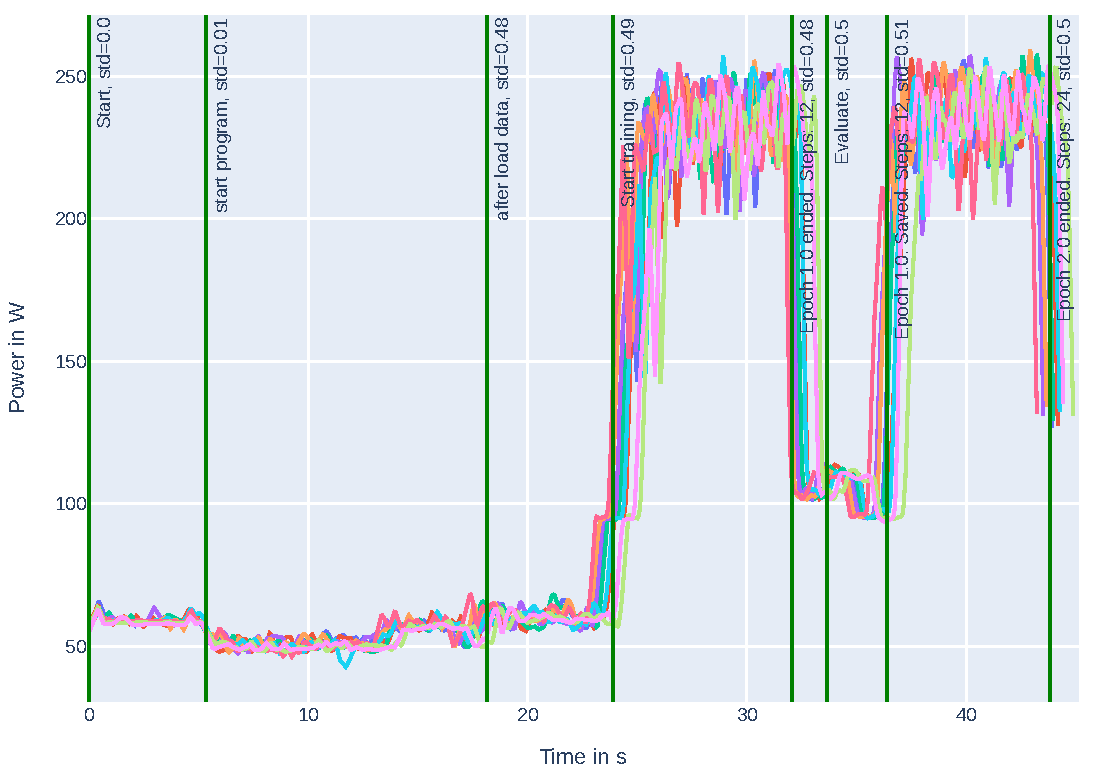
\includegraphics[width=\linewidth]{power-measurements/stacked_plots/roberta_stop_without_saving.pdf}
    \caption{Power draws of the ML up until stopping after epoch 2}
    \label{fig:plot_partial_abort_stacked}
\end{figure}

\begin{figure}
    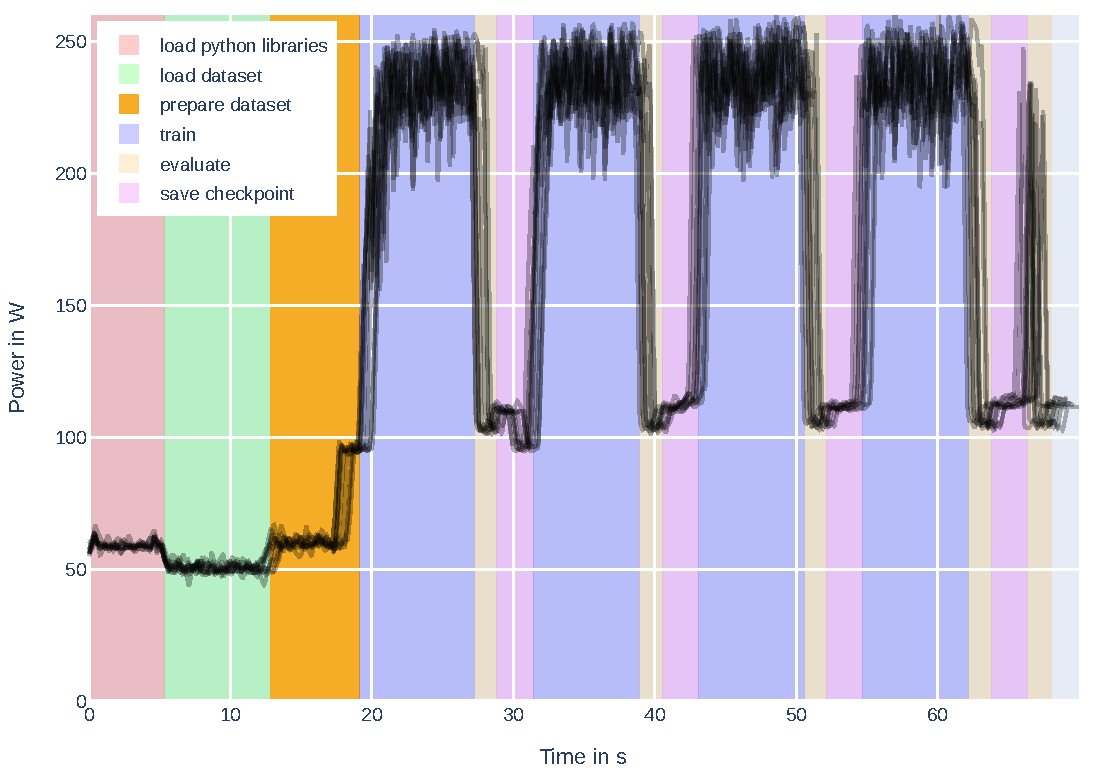
\includegraphics[width=\linewidth]{power-measurements/stacked_plots/roberta_continue_after_not_saving.pdf}
    \caption{Power draws after continuing from the second checkpoint}
    \label{fig:plot_partial_abort_continue_stacked}
\end{figure}

\paragraph{Calculating the energy costs of each run}

The energy costs of each experiment are contained in Table \ref{tab:experiment_overhead}.

\begin{table}[h!]
    \centering
    \begin{tabular}{|c|c|c|}
    \hline
        Experiment & average energy cost & standard deviation \\ \hline
        \ref{experiment:full}, whole run &  12.97 kJ & 0.04 \\ \hline
        \ref{experiment:partial_checkpointed}, suspend after checkpoint and resume &  13.94  kJ & 0.1 \\ \hline
        \ref{experiment:partial_checkpointed_aborted}, abort early and resume &  15.72 kJ & 0.07 \\ \hline
    \end{tabular}
    \caption{Environment parameters of the power measurements}
\label{tab:experiment_overhead}
\end{table}

\section{Introduction of \modelname}

Now that we know what a high-level job looks like, we can pick it apart and reduce the real-world measurements of one program to a more generic model. 

Summarizing the findings from the previous paragraphs; it was shown that 

\begin{itemize}
    \item The given job has phases that have different power draws
    \item Checkpointing \& resuming carries overhead in the form of startup costs and possible wasted work.
\end{itemize}

The parameters for the improved job model are shown in form of the python implementation in Listing \ref{listing:model_python}.

\begin{minipage}{\linewidth}
\begin{lstlisting}[language=python, frame=single, numbers=none, caption={Python Model definition}, basicstyle=\ttfamily, label={listing:model_python}]
class ModelParameters(TypedDict):
    startup: List[Phase]
    work: List[Phase]
    
class Phase(TypedDict):
    name: str
    duration: float
    power: float
    is_checkpoint: NotRequired[bool]   
\end{lstlisting}
\end{minipage}

Some simplifications are made: the duration of each phase is well known and the power per phase is a constant. 
Phases can also be named for later reference.
These phases essentially define a step function, i.e. piecewise constant function.
Unlike a traditional step function, the start- and endpoints of each "piece" would be encoded implicitly by the previous phases.
Using these specifications, a simple time-to-power function can be defined, that looks up the input time and traverses the phases in order.

Initially, we considered allowing any expression instead of a constant value for power and then using Python's \verb|evaluate()| to e.g. allow a function-per-phase model.
In Section \ref{sec:checkpoint_resume_lp}, having a rather restrictive step function will be of advantage, however. \todo{Add some more explanation to this in that section}

The measurements that have been taken can now be fit into this new model. 
As each measurement-point can be associated to a phase via the aforementioned added logging, the average of each phase-associated measurement is used to determine the model parameters. 
The durations of the phases are calculated similarly by taking the average time the logging occurred at during the measurements.

Using this strategy on the 10 complete runs results in Figure \ref{fig:model_overlaid}, which shows the derived model in black with the previous Figure \ref{fig:plot_full} in less opacity. 
The startup phase looks well approximated, visually however there is some error during the work phases.
The training phases each have a high variance, which is not captured by the constant power approximation. After each training  phase, the power goes down seemingly linearly, which is also approximated by the constant.

One notable point, this model is a superset of the previous constant-no-overhead model used in the related work.
Previous jobs can be modeled with just one phase of work, resulting in a constant power over its execution. Leaving the startup phases empty creates no overhead on resuming.

\todo{Should probably add the phase markers back in}
\begin{figure}
    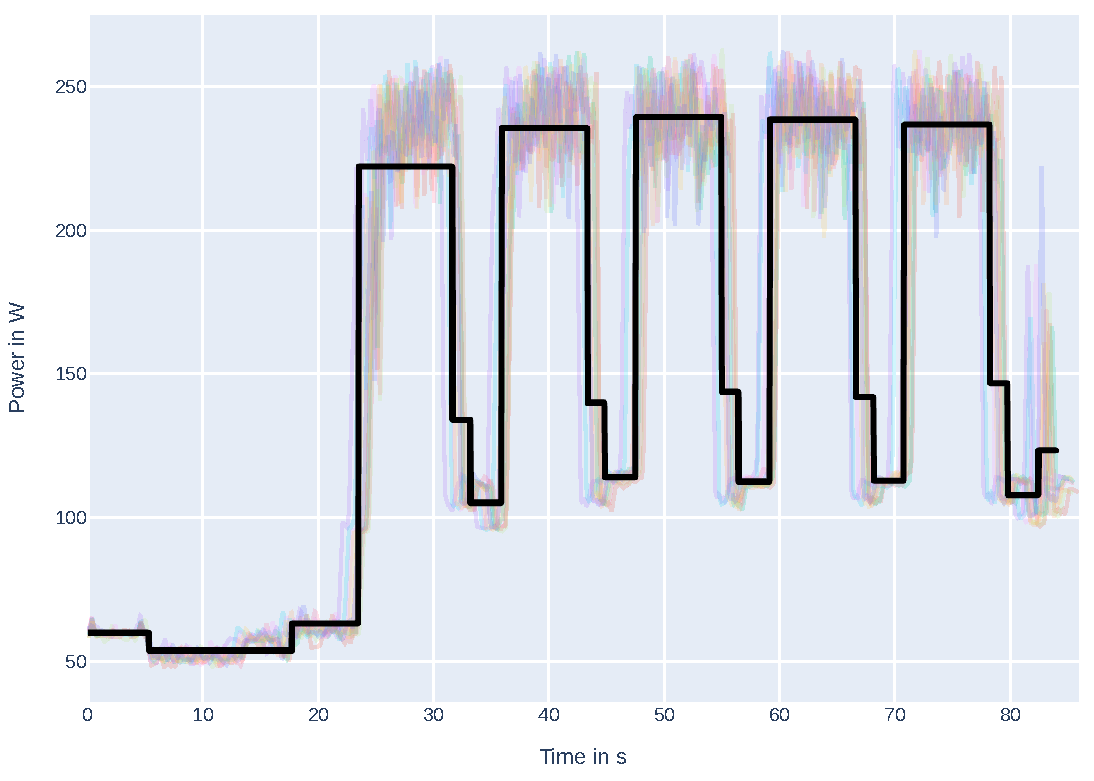
\includegraphics[width=\linewidth]{power-measurements/model_overlaid.pdf}
    \caption{Model of roberta.py (black) vs. the measured runs}
    \label{fig:model_overlaid}
\end{figure}

\paragraph{Model Error Analysis}

To analyze the error of this model, we cross validated the power's RMSE and the total energy using \verb|scikit-learn|'s \verb|LeaveOneOut| strategy. 
The first one would give a measure of the model's accuracy on a short-time (sub-second) scale, the latter would  tell the long-time (whole job) scale accuracy of the model.

Each of the 10 runs would be taken as the ground truth while the other 9 would be used to create the model. 
The results are the following: the power between the prediction and remainder has an RSME of 39.3 W while the difference in total energy is calculated as -0.1 kJ. 

Interpreting this, it seems that the model performs poorly as a predictor of the exact power used at some time point as the RMSE is rather large (think of the maximum power drawn being about 250W). 
However, in the context of carbon aware scheduling, this should not be too big of an issue as the time frames for carbon-emissions are orders of magnitudes larger (\emph{electricitymaps} has a resolution of 1 hour for carbon emissions intensities). 
The high error likely comes from the high variance during the training phases which is not captured in the model.

The total energy predicted by the model is very close to the actual real life experiment, this should mean that the total carbon calculated on the model should also be close to the carbon emitted by the real program.

	\chapter{Implementing Schedulers using the New Model}

Now that an improvement on the job model has been made, the question, on how to evaluate the implications of said model, remains. 

% We first need to explain why we chose our approach (building upon exisiting work inside GAIA). The other option that is not using a simulation would be to schedule real jobs, for example by creating a Slurm plugin.

% We can then evaluate how well a Slurm plugin would work for our given Forschungsragen. End that section by deeming the plugin idea as unfit, we can then shift to arguing for the simulation approach as that is also something that just came out in related work (perhaps we should see wether we list GAIA as related work or introduce it just then)

\section{Choosing an Implementation Approach}

\subsection{Carbon-aware scheduling via a Slurm plugin}
\label{subsec:slurm_plugin}

My first idea was to use a non-simulation approach. 
The HPI's Data Lab \footnote{\url{https://hpi.de/forschung/infrastruktur/hpi-data-engineering-lab.html}} runs a \emph{Slurm} cluster and also has some nodes with power measurement infrastructure included. 
Slurm is an "open source, fault-tolerant, and highly scalable cluster management and job scheduling system for large and small Linux clusters"\footnote{\url{https://Slurm.schedmd.com/overview.html}}. 
The job scheduling part is important here, it also supports a plugin infrastructure that includes scheduling plugins. 
One of the highlighted papers\cite{inigo_goiri_greenslot_2011} in the related work section specifically used Slurm for its carbon-aware scheduler implementation and thus seemed like a good starting point for my own work.

\paragraph{Installing Slurm locally}

For my purposes, a local installation would suffice as I would not need to run heavy workloads but instead just the scheduling part of Slurm. 
While there is a Slurm \verb|apt get| package for my Ubuntu version, this would not work as any plugins to be included during the Slurm compilation, meaning I would have to do the same.

Slurm's documentation provides some guidelines on how to install Slurm, which I followed. 
I tried cloning the main branch, but I got stuck during the compilation process. However, using the predefined released versions worked.

Installing \verb|munge|\footnote{\url{https://github.com/dun/munge/wiki/Installation-Guide}} is also necessary, which is used for authentication in Slurm.

One problem arose as I tried to start the \verb|Slurmd|- and \verb|Slurmctld| services. The first one is the worker service that would later execute jobs submitted to Slurm. The latter is the main controller that, for example, schedules jobs on workers. While the command to start them would not fail, upon node inspection via Slurm's \verb|scontrol| command, it would show that all nodes are \verb|DOWN| instantly.
|
Dealing with Slurm's problems usually leads to inspecting its logs, in my case the logs showed the following:

\begin{lstlisting}[language=bash, frame=single, numbers=none, caption={Slurm error logs}, basicstyle=\ttfamily]
$ less config.log

error: Couldn't find the specified plugin name for cgroup/v2
    looking at all files
error: cannot find cgroup plugin for cgroup/v2
error: cannot create cgroup context for cgroup/v2
error: Unable to initialize cgroup plugin
error: Slurmd initialization failed

\end{lstlisting}

Slurm uses Linux' \verb|cgroup| feature to manage the submitted job's hardware ressources. The log hints at some problem related to Slurm's usage of it.
The solution was this was to provide Slurm's \verb|cgroup.conf| file. In my use-case of getting Slurm to simply start, this did not need to be very sophisticated so I just used an off-the-shelf (off-the-stackoverflow\footnote{\url{https://stackoverflow.com/a/74211989}}) configuration file.

Running \verb|scontrol| again, I was finally able to see idling nodes, meaning that Slurm was successfully installed form source:

\begin{lstlisting}[language=bash, frame=single, numbers=none, caption={Slurm running}, basicstyle=\ttfamily]
$ scontrol
scontrol: update NodeName=vincent-Laptop STATE=RESUME
\end{lstlisting}

\paragraph{Creating a scheduler plugin}

The Slurm documentation provides a short guide on how to add a plugin to Slurm.\footnote{\url{https://Slurm.schedmd.com/add.html}}. 
As a start, I simply copied Slurm's default scheduler (which is also a plugin) to to the specified directory under a new name, and addings that new name to Slurms build files. 
It was then was time to recompile Slurm. 
Now however, during the recommended \verb|autoreconf| step, an error occured:

\begin{lstlisting}[language=bash, frame=single, numbers=none, caption={Plugin recompilation errors}, basicstyle=\ttfamily]
$ autoreconf
auxdir/x_ac_sview.m4:35: warning: macro 'AM_PATH_GLIB_2_0' 
    not found in library
configure:25140: error: possibly undefined macro: AM_PATH_GLIB_2_0
      If this token and others are legitimate, 
      please use m4_pattern_allow.
      See the Autoconf documentation.
autoreconf: error: /usr/bin/autoconf failed with exit status: 1
\end{lstlisting}

The solution, while not very obvious, was to install the \verb|libgtk2.0-dev| library. \footnote{\url{https://stackoverflow.com/questions/7805815/autoconf-error-on-ubuntu-11-04}}. 
I then added a simple logging which then showed up in Slurm's log files too.

\paragraph{Adding more logic to the scheduler plugin}

One very helpful step for developing inside Slurm is to enable the debugging flags.
This must be decided before compilation by using the \verb|--enable-developer| and \verb|--disable-optimizations| flags during the \verb|/configure| step. 
With that, debug symbols are added to the outgoing binaries. 
As I was using vscode, I could then attach its debugger to the running Slurm thread with full functionality.

The code of the plugin runs in its own thread and there is no sandboxing or similar around it.
Thus there are seemingly no limitation on what can be done inside the plugin. 
For testing, I read out information on the incoming jobs such as set constraints or the user supplied comments. Terminating the jobs was also possible inside the plugin.

\paragraph{Problems of a scheduler plugin}

One big problem manifested in that not all jobs "showed up" inside the plugin's job queue. 
If I would submit 6 jobs, via Slurm's \verb|squeue| command, only a part such as the last 3 could be logged inside the plugin.
A possible explaination for this could be Slurms scheduler architecture: while there is a scheduler plugin, there also is a scheduler inside Slurm's main loop. 
That main scheduler loop also uses the same job queue as the plugin.

To hack around this, I tried disabling Slurm's main scheduling loop by setting \verb|sched_interval=-1| inside the Slurm configuration file. 
While this had the effect of being able to access all incoming jobs inside the plugin, it also had the side-effect of disabling all logic concerning starting the jobs.
So by choosing this route, the plugin would apparently also need to re-implement alot of extra logic, which conventionally would be not be put inside the scheduler plugin. 

I also looked into whether there were any API hooks that are exposed to the plugin. 
Up until Slurm version 20.11, scheduler plugins had callbacks such as when jobs were submitted. There also was support for "passive" scheduler that would get invoked when determined by Slurm.
The version I tested however,  23.11, removed all such functionality and documentation. All plugins are implemented via threads that only have callbacks on when they are started and stopped.

Thus, since there was no apparent way of getting around this scheduler race condition between the plugin and the main loop. 
The scheduler approach as a whole was dropped. 
While I would not say that a plugin approach is impossible, the effort to implement one from scratch subjectivly seems very high. 
The public documentation for developing on Slurm is scarce. 
There is a mailing list that can be searched, but it looks to be mostly aimed for administrating Slurm and not developing it.

Other avenues that could be explored are Slurm's Lua plugins. There is also a \emph{Slurm simulator}\footnote{\url{https://hpckp.org/articles/how-to-use-the-Slurm-simulator-as-a-development-and-testing-environment/}} which could potentially be used for carbon-aware scheduling simulation, but that I did not look into much for reasons of little documentation and seeming lack of continued support.

\subsection{Using a Simulation approach}

Thankfully, just at that time, a new paper \cite{hanafy_going_2024} was released. 
They made a prototype testbed for simulating job scheduling on cloud providers. These Jobs could be executed on spot instances (cheap VMs that seek to increase cloud utilization), on-demand instances (short-notices VMs that are thus more expensive) or pre bought VMs (medium cost, but may be wasted), the paper then discussed balancing carbon- and dollar costs. 
They included a small notion notion of hardwre requirements in the form of required CPUs per job, but that was only used to scale the cost; all hardware requirements were abstracted away in the form of the cloud always having computing ressources available.

The important part is that they also included an implementation of some schedulers used in the highlighted related works. Among that an implementation for WaitAWhile\cite{wiesner_lets_2021}.
This meant that I could add the improved job model to that exisiting testbed and have something to compare against aswell.

\paragraph{Description of the GAIA simulator}

I would first like to describe the existing testbed in detail to make it clear which part is my work and which is not. A class diagram is provided in \ref{fig:class_diagram} which is heavily inspired by the existing architecture diagram in the original paper. 

\begin{figure}
    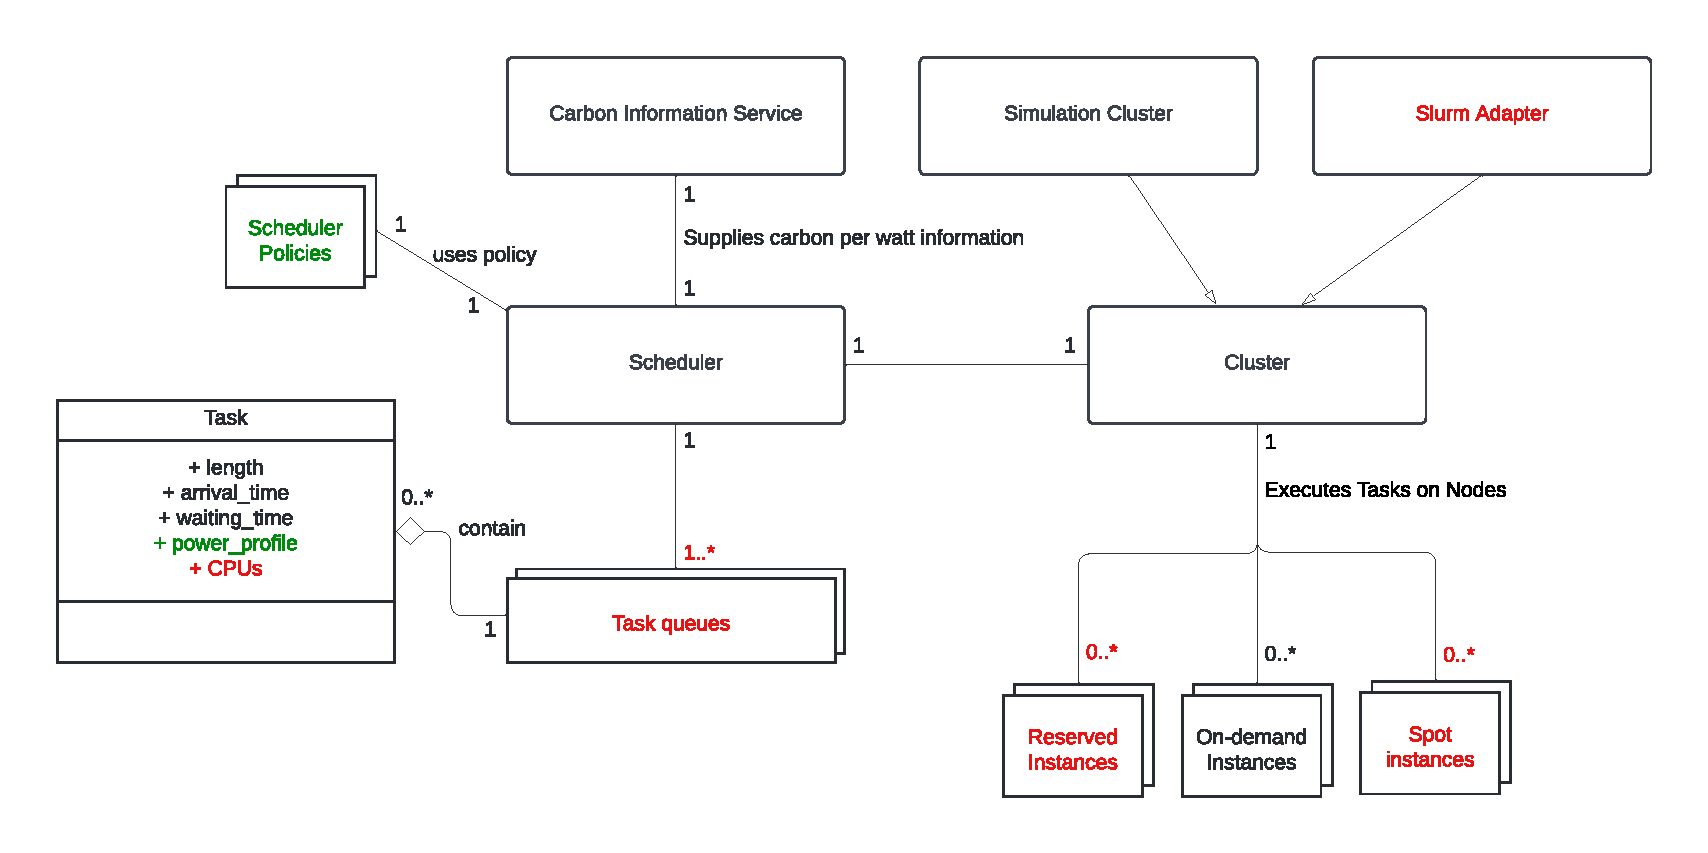
\includegraphics[width=\linewidth]{images/MA Thesis Diagram.pdf}
    \caption{Class Diagram of GAIA, red indicates removal or reduction, green indicates additions}
    \label{fig:class_diagram}
\end{figure}

The main part of GAIA is the scheduler. At program start, it takes parameters\todo{I should probably give an overview of which parameters are supported, so I have that terminology later} that determine the scheduling, such as whether tasks can be interrupted, how to use the carbon information (e.g. use a perfect-information / oracle approach or to use a running average), and how to balance the dollar cost for scheduling. 
The latter I removed for simplicity, which is marked in the figure via the red color of the reserved and spot instances. In my case of carbon-aware scheduling, I did not need that feature.

In the original implementation, the scheduler had multiple queues of tasks. 
The paper presented an approach of a short queue (tasks under 2 hours) and long tasks (all other), short tasks would get scheduled on spot instances. 
Again, as I already removed the spot instance, feature, I did not need the queue multiplicity and it was removed.

The tasks queues are based on historical traces. GAIA provided multiple traces that are described in the paper. To those I added a trace of the HPI's Data Lab, which will be analysed in section\todo{Link this}.

Tasks have a predetermined length (as saved in the trace), and they also hold some data that is used for scheduling such as their arrival time in the system, and how long they should wait until execution. 
Some properties such as required CPUs were removed.
My contribution of the phases-and-power model was added to the tasks.

The Scheduler policies are also marked green, as I added scheduler policies that could use this new model. Specifically, I added a (non-) checkpoint \& resume scheduler that works on oracle carbon prediction, this will be further explained in the latter sections.

Scheduled Tasks are submitted to a cluster.
In my case, this is a simulated, already implemented, cluster that simply logs when each task is entered and finished. 
In the original paper, they also used an open source adapter that would submit the tasks to an actual Slurm cluster. 
While this approach could have been used, I decided against it on the basis of not adding further complexity. 
Thus I also removed the Slurm adapter from my implementation.

% \paragraph{Data being used}
% 
% here i could describe which data is already being used (the traces, aswell as the historical carbon data)
% \begin{itemize}
%     \item Welche Traces gibt es, wodurch werden die characterisiert? (Länge, Anzahl, etc, etc) Vllt. kann man hier nen coolen vergleich erstellen, Auch könnte man ein paar Sätze darüber schreiben, wie die bisher in GAIA aufgenommen wurden.
%     \item Wie den scorelab trace benutzen und übersetzen? Gerne auf ner halben Seite aufschlüsseln, was die einzelnen Attribute aus sacct bedeuten.
%     \item Ansonsten kann man noch die dynamic ernergy sachen als Datenquelle auflisten, bzw. das mini experiment mit fmnist und roberta 
% \end{itemize}

\section{Implementing simulation-schedulers using the new model}

I would first like to summarize assumption that GAIA makes on the problem of carbon aware scheduling:

\begin{enumerate}
    \item job lengths are known
    \item all considered jobs are batch jobs and can thus be shifted temporally based on user deadlines
    \item carbon information is provided for near future time spans, no error is considered
    \item there are no hardware limitations or considerations, all jobs are executed in an isolated manner
    \item jobs have a constant power draw and can be checkpointed \& resumed for free
\end{enumerate}

Especially the last point will be modified going further. As shown in section \ref{sec:improving_the_model}, jobs now have a predefined, variable power draw according to the defined phases. Resuming a job also carries an additional startup phase with it.

\subsection{Modifying the existing jobs to use the new model}

The first step to be taken was to add the described model to the jobs as outlined in figure \ref{fig:class_diagram}. 
So far, jobs were generated from \verb|csv|-formatted traces, one example being provided in listing \ref{list:trace_csv}.

\begin{lstlisting}[frame=single, numbers=none, caption={Excerpt from the Alibaba-PAI trace}, label={list:trace_csv}, basicstyle=\ttfamily]
arrival_time,   length,     cpus
0.0,            6302.0,     1
68.0,           1000.0,     1
463.0,          1570.0,     3
838.0,          23549.0,    1
\end{lstlisting}

In the original GAIA implementation, jobs have a \verb|arrival_time|, which signify when the job should be added to the simulation in seconds. 
The \verb|length| of a job similarly encodes the seconds a job needs to fully execute. The \verb|cpu| column was not interesting for my work, as previously discussed.

The chosen way of supplying the model information was to add two new columns to the trace files, which would entail the type of job and a column for arguments. 
As of now, the following types are supported: \verb|constant|, \verb|mocked-constant-from-phases|, \verb|phases|, and \verb|ml|. 
The first two \verb|constant| types are for backward-compatibility with GAIA, and would be used in the evaluation later. 

Type \verb|phases| is the main way of creating a job with phases such as the one used in the experiment. The supplied argument in that case would entail a python readable \verb|dict|, essentially a \verb|JSON|-like definition of the model as described in listing \ref{listing:model_python}.
As this was just a string, I would then use Python's \verb|eval()| to read it back into a python object.\todo{Check how and if I should visualize this}
As an example, a simplified \verb|roberta.py|, the job that was measured in section \ref{sec:power_measurements}, could look like the code in listing \ref{list:roberta_model_definition}

\begin{lstlisting}[frame=single, numbers=none, caption={Simplified definition for a job similar to the experiment}, label={list:roberta_model_definition}, basicstyle=\ttfamily]
{
    'startup': [
        {'name': 'Start', 'duration': 5.34, 'power': 59.9},
        {'name': 'Finish Imports', 'duration': 12.36, 'power': 53.77},
        {'name': 'Data loaded', 'duration': 5.75, 'power': 63.17}, 
    ],
    'work': [
        {'name': 'Train', 'duration': 8.17, 'power': 221.93}, 
        {'name': 'Evaluate', 'duration': 1.54, 'power': 134.0}, 
        {'name': 'Save', 'duration': 2.72, 'power': 105.1,
            'is_checkpoint': True}, 
    ] * 5
}
\end{lstlisting}

In order to use this model definition and read out the power of a job at a given time, a function was crated that essentially traverses all phases in order, keeping track of the time, and returning the power of the phase when the requested time is reached. 
This was also used to create figure \ref{fig:model_overlaid}.

A generalizing helper type is \verb|ml|, which takes a dictionary of parameters and converts that to model parameters for the \verb|phases| type. A similar job as to the one above would be created with the following:

\begin{lstlisting}[frame=single, numbers=none, caption={Generic model definition for machine learning jobs}, label={list:roberta_model_definition_generic}, basicstyle=\ttfamily]
{
    'start_duration': 23.45
    'start_power': 60
    'training_duration': 8.17
    'training_power': 221.93
    'evaluate_duration': 1.54
    'evaluate_power': 63.17
    'save_duration': 2.72
    'save_power': 105.1
    'epochs': 5
}
\end{lstlisting}

\subsection{Uninterrupted oracle scheduling} \label{sec:uninterrupted_oracle_scheduling}

There already was an existing version of this scheduling approach which assumed constant power and that the carbon trace would be fully known ("oracle"). 
Jobs would not be able to checkpoint \& resume in this version.
The algorithm for which is pseudocoded in listing \ref{list:pseudocode_oracle}.

\begin{lstlisting}[frame=single, numbers=left, caption={Pseudocode for the original non-interrupt oracle scheduler}, label={list:pseudocode_oracle}, basicstyle=\ttfamily]
function schedule_job_no_checkpointing_resuming(job):
    possible_starts = []
    for every possible starttime until deadline:
        calculate carbon_emissions_of_job at starttime
        add carbon_emission to possible_starts
    
    return starttime with least carbon emissions

function carbon_emissions_of_job(job, carbon_trace):
    sum_of_emissions = 0

    for each second of job:
        sum_of_emissions += carbon_trace at timepoint * constant_watt
    
    return sum_of_emissions
\end{lstlisting}

In order to adjust this to the new model where power is a function of time, only line 13 needed to be changed. 
Thus, I implemented a python function whose input is the model parameters (see listing \ref{roberta_model_definition}), and which would return the power at a specified time. 
Evaluating this scheduling approach will take place in section \ref{sec:evaluate_scheduling}, after another scheduling algorithm is introduced.


\subsection{{Checkpoint \& resume scheduling for heterogeneous jobs}} \label{sec:checkpoint_resume_lp}

Under the constant-power, no startup-overhead assumption of the already existing implementation, the algorithm for this scheduler worked like the following:

\begin{itemize}
    \item order all time slots until the job deadline by their emissions ascending
    \item execute the job on those time slots until done
\end{itemize}

This would minimize the carbon emissions, as only the best time slots would be used, but would also create unrealistic schedules sometimes. 
For example, in figure \ref{fig:schedule_problems}, if a job's deadline is in the distant future, due to the diurnal nature of the electric grid, the job would be scheduled on the "peaks" of each day. Sometimes this would lead to a job being simulated as being executed for very short timeframes at a time\todo{Check wording}. As shown in the power measurement chapter, this kind of scheduling would create a lot of overhead from starting so many times.

\begin{figure}
    \missingfigure{I should show a Gantt chart of the mishappen scheduling for the checkpoint resume scheduler}
    \caption{Problems in the checkpoint \& resume scheduling under the previous assumptions}
    \label{fig:schedule_problems}
\end{figure}


In order to implement a scheduler for the improved job model, I chose to use \emph{linear programming} (also: LP).
In a nutshell, LP is an optimization method, that given linear equations and constraints, finds a set of variables (or a vector) that would minimize (or maximize) an optimization goal. 
The reason for choosing this approach over, for example coming up with a "standard" algorithm, was that I had never used LP before and that due to the "inherent optimization", the burden of\todo{Kann man das so sagen?} proof for the correctness would be lower.

Translating this to the context of carbon-aware scheduling, the resulting vector would decode when a job should be executed, the optimization goal would be to minimize the emitted carbon. 
A constraint for example could be that all time slots being executed should add up to the job length. 
The big challenge is then to model all of this in the form of mathematical equations, which will be most part of this section's remainder.

\paragraph{Personal experience with linear programming}

Linear programming is its own programming paradigm. Unlike, for example, imperative programming, where each instruction would be coded explicitly, enabling classic debugging and such, in LP, a mathematical model would be written which is then solved by a \emph{solver}. 
Different implementations for these solvers exist, but atleast in my case, the result output by a solver would either be an error, or the result set. 
As the solver uses the whole model simultaneously, "debugging" individual parts of the model is not possible outside removing them from the overall model.

Thus, an iterative approach to LP proved useful. 
I would encode some part of my overall problem into the model, solve it, and immediately plot the variables of the result set and check them visually.
The visual check is very important. 
Many times the solver would solve the problem "so well" that jobs would get scheduled in a way that the emitted carbon is minimized, but the jobs would be executed in edge cases that I did not intend, but that are possible under the model, examples of this will be given in the following parts.

Another part of programming LP is "just knowing the tricks". 
Many common programming operations, especially ones for control flow, cannot be expressed directly (as they need to be a linear equation).
There are some mappings for such operations, but finding out how seems to be harder than in other paradigms, since the LP community appears to be smaller in comparison and online resources are limited.
Some "tricks" will be highlighted in the latter parts as well. 

\paragraph{Modelling carbon-aware scheduling in a linear program}

In this part, I would like to preset the steps taken to model the scheduler as an LP problem, highlight some implementation details and visualizing the results of each step.
I used python's \verb|PuLP| library.
It allows creating LP models to standard file types and also helps in calling external solvers as well as querying the results.

\subparagraph{Executing the job}

Firstly, as the job has a certain length and a set deadline, I chose to use an array of time slot-variables as my result set. Each such variable would be a boolean signifying whether the job would be executed at that time.
For the first constraint, the sum of all boolean variables (which are represented as 0 and 1) should add up to the job length, effectively executing the job for length-many time slots.
The necessary objective function is to be defined as each time slot-being-executed multiplied by the carbon-per-watt at that time slot.

As an example, the code for this is shown in listing \ref{fig:lp_work}.

\begin{lstlisting}[frame=single, numbers=left, caption={LP Implementation for basic scheduling}, label={list:lp_work}, basicstyle=\ttfamily]
prob = LpProblem("CarbonAwareScheduling", pulp.LpMinimize)
work = LpVariable.dicts("work", (t for t in range(DEADLINE)), cat="Binary")

prob += lpSum([work[t] * carbon_cost_at_time[t] for t in range(DEADLINE)]) 
prob += lpSum(work[t] for t in range(DEADLINE)) == WORK_LENGTH

solver = pulp.Gurobi_CMD(timeLimit=timelimit)
prob.solve(solver)
\end{lstlisting}

The first line creates an LP problem and defines the optimization goal to be a minimizing one. 
Then, a variable "work" is defined as being \verb|DEADLINE|-many (in this case 300) integer-indexed boolean variables. 
These will be modeled as the time slots.
Line 4 defines the optimization goal; each time slot will be multiplied by the carbon emitted there. As one factor is a boolean, this will only increase the sum if the time slot is scheduled. 
The last two lines start the solving library. 
\verb|PuLP| offers an open source solver by default, but during development this proved to be very slow and also did not offer features such as time limits and retrieving intermediate results.
I thus chose the \emph{Gurobi} solver, a commercial solver that also offers academic licenses. 
That one supported the previously lamented features and increased development time by a lot. 

The running example will be a deadline of 300 time slots, the job has a startup phase of 20 units and has 100 work units. 
The above code leads to a result set that is visualized in figure \ref{fig:lp_work},
which on the bottom part shows the carbon emissions at each time slot and the upper graph shows the chosen time slots.
Looking at the figure, the results are not too surprising: the chosen time slots are just the points where emissions are lowest, essentially being equal to the result of the WaitAWhile-Algorithm.

\begin{figure}
    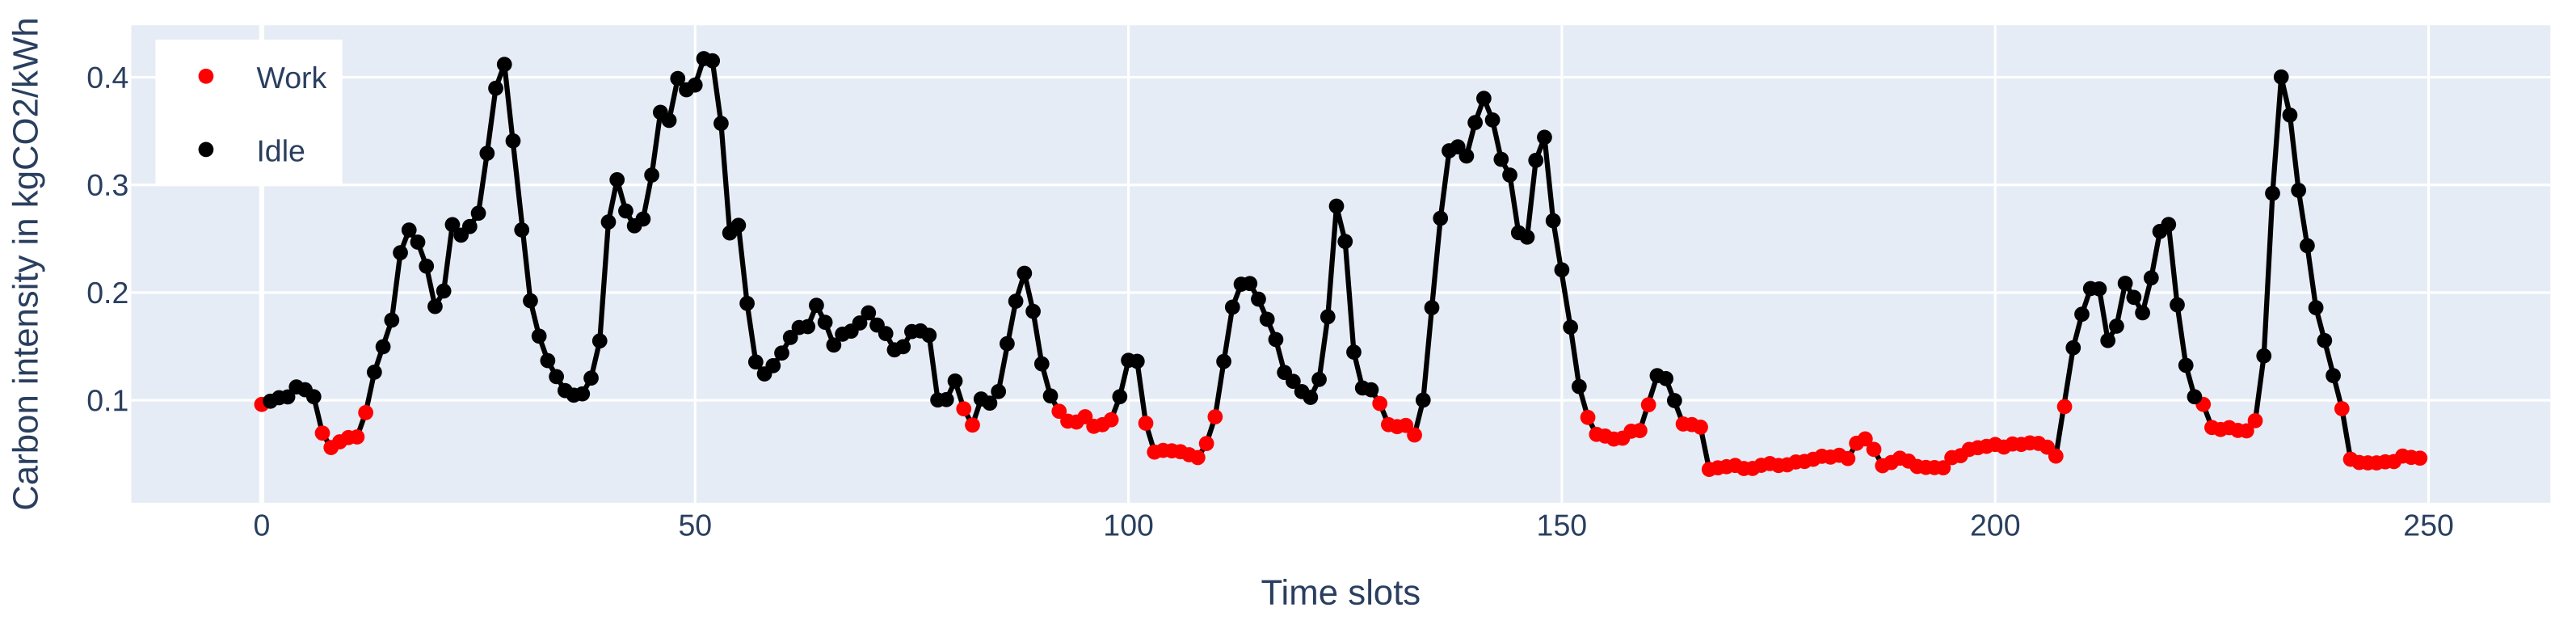
\includegraphics[width=\linewidth]{GAIA/notebooks/lp_work.pdf}
    \caption{Visualizing the result set of executing the job for its length}
    \label{fig:lp_work}
\end{figure}

\subparagraph{Adding overhead via startup phases}

In order to add a cost to starting a job, the code following in listing \ref{list:lp_overhead} is complemented, some parts are excluded for brevity.

\begin{lstlisting}[frame=single, numbers=left, caption={LP Implementation for overhead}, label={list:lp_overhead}, basicstyle=\ttfamily]
for t in range(DEADLINE - 1):
    prob += startup_finished[t] >= work[t + 1] - work[t]
    prob += startup_finished[t] + work[t] <= 1
    prob += starting[t] + work[t] <= 1

for i in range(STARTUP_LENGTH - 1, DEADLINE):
    prob += pulp.lpSum([starting[i - j] for j in range(STARTUP_LENGTH)]) 
        >= STARTUP_LENGTH * startup_finished[i]
\end{lstlisting}

In this snippet, two extra dictionary-variables are introduced, \verb|startup_finished| and \verb|startup|.
For every time slot (line 1), set \verb|startup_finished| to true if and only if there is a 0 to 1 transition along the \verb|work| dictionary. This becomes apparent when looking at the following truth table \ref{tab:truth_table_startup_finished}.
Notice how the numerical booleans help in this case, as negative integers get mapped to \verb|0|, or \verb|false| respectively.

\begin{table}[h!]
\centering
\begin{tabular}{|c|c|c|c|}
\hline
    $work[t]$ & $work[t+1]$ & $work[t+1]$ - $work[t]$ & $startup\_finished[t]$ \\ \hline
    $0$ & $0$ & $0$ & $0$ \\ \hline
    $0$ & $1$ & $1$ & $1$ \\ \hline
    $1$ & $0$ & $max(-1, 0) = 0$ & $0$ \\ \hline
    $1$ & $1$ & $0$ & $0$ \\ \hline
\end{tabular}
\caption{Truth table for finding when working time slots begin}
\label{tab:truth_table_startup_finished}
\end{table}

Line 3 and 4 ensure that "working" time slots and "startup" time slots are mutually exclusive.
The last loop defined that if (\verb|* startup_finsihed[i]|) a startup must be finished by some time slot, the previous \verb|STARTUP_LENGTH|-many time slots must be used for starting the job.

At this point, the solver scheduled jobs in a way that would sometimes execute the job at the very first time slots, as no startup could happen before time slot $0$, thus minimizing carbon but obviously producing a bogus result.
I thus added an extra constraint that work can only be scheduled after atleast the length of the startup phase.
The emitted carbon goal is changed to also include these new startup time slot, similarly to the previous listing \ref{list:lp_overhead}.
With this step, the result already looks more like a reasonable schedule, as shown in figure \ref{fig:lp_overhead}. 
This time, the optimal schedule includes executing the job in one go.
Doing a visual check, the job is also executed on seemingly the lowest carbon intensities.

\begin{figure}
    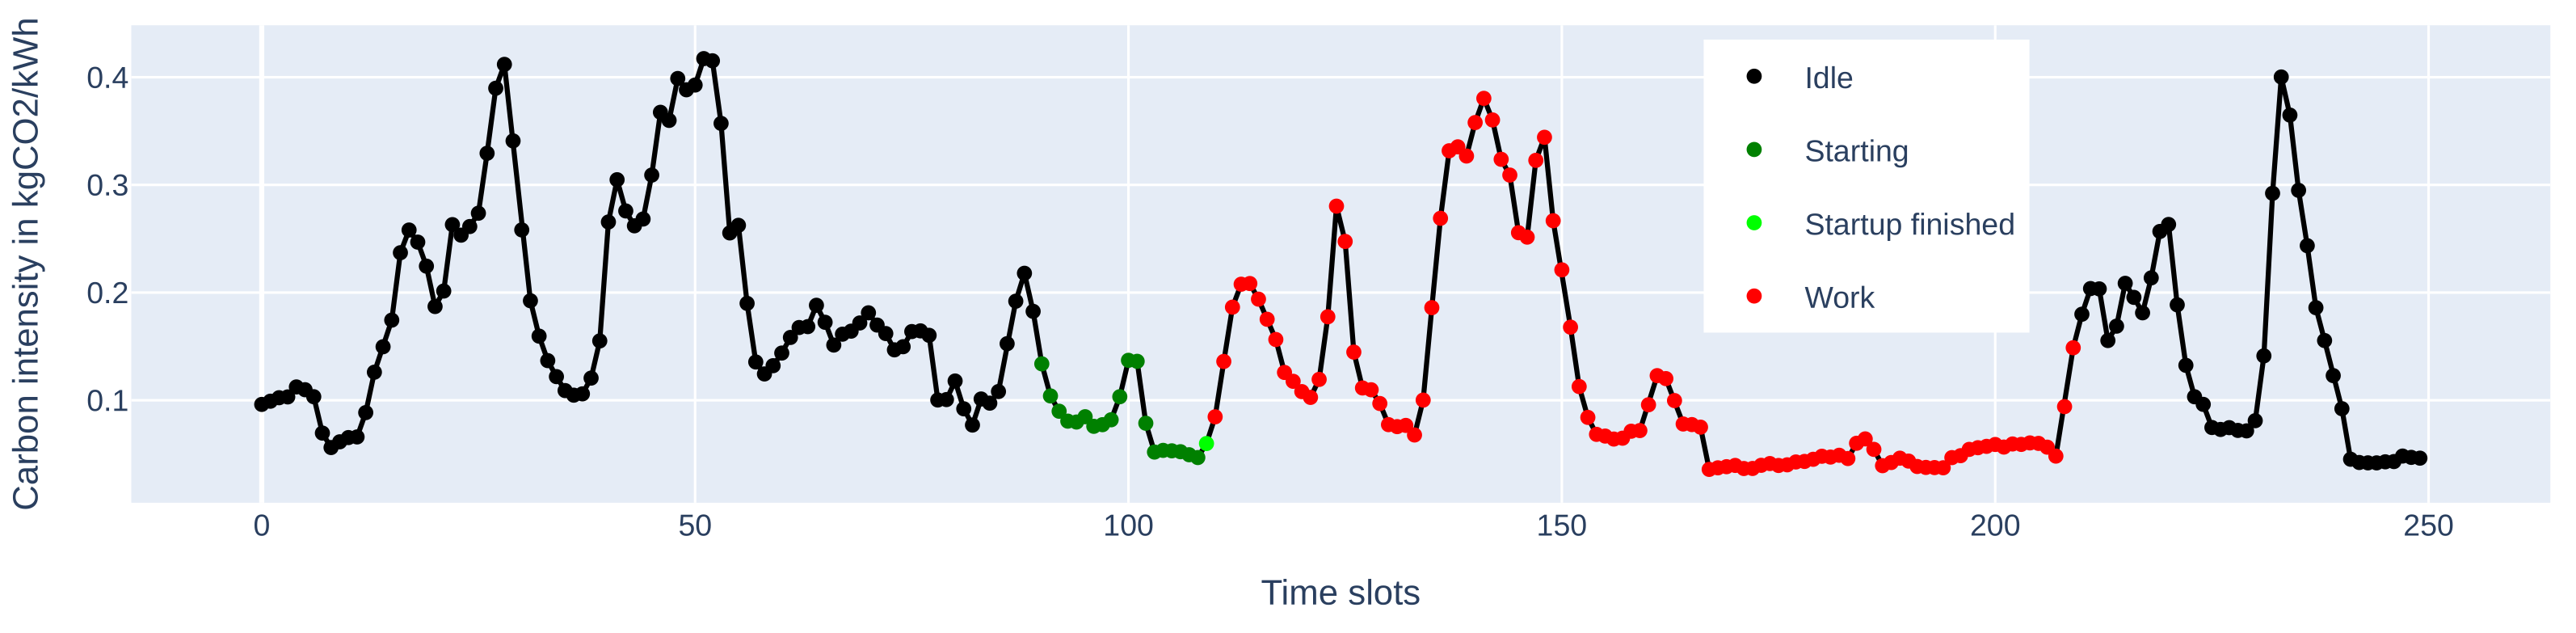
\includegraphics[width=\linewidth]{GAIA/notebooks/lp_overhead.pdf}
    \caption{LP Scheduling with overhead in form of a startup phase}
    \label{fig:lp_overhead}
\end{figure}

\subparagraph{Adding a notion of progress}

So far, the assumption of constant power has been continued.
Changing this assumption under the previous other scheduler using the greedy algorithm in section \ref{sec:uninterrupted_oracle_scheduling}, was relatively easy, as changing the constant expression to python function of the model sufficed. 
This cannot be reused in LP however, as the problem definition may only include linear equations, which a generic function is not. 
In order to add dynamic power into the linear program, I decided to \emph{linearize} the function, meaning the model needed to be split up into multiple linear approximations.

As the model already is essentially a step function of time to power, each phase being one step, the mapping is inherently pretty close. 
As such, \emph{a lot} of equations were needed that each express "if the progress in the job is $t$, set power to $model(t)$". 
For that a notion of progress and time is needed inside the model.
The progress inside each startup-phase needs to reset, as that can happen multiple times during the schedule. 
On the other hand, the progress for the productive work must not be reset between execution blocks. 

I added the following code to express this:

\begin{lstlisting}[frame=single, numbers=left, caption={Progress Variables in LP}, label={list:lp_progress}, basicstyle=\ttfamily, breaklines]
# define "work_time_progressed" and "startup_time_progressed" as 
# DEADLINE-many integer variables

M = DEADLINE * 2
for t in range(DEADLINE-1):
    if (t>0):
        prob += startup_time_progressed[t] >= startup_time_progressed[t-1] + 1 - (1 - starting[t]) * M 
        prob += startup_time_progressed[t] <= startup_time_progressed[t-1] + 1 + (1 - starting[t]) * M
    prob += startup_time_progressed[t] <= starting[t] * M 
    prob += work_time_progressed[0] == 0
    if (t > 0):
        prob += work_time_progressed[t] == work_time_progressed[t-1] + work[t]
\end{lstlisting}

On a base level, the idea is to count up each progress variables by 1, if a time slot is being determined for work or startup respectively (see line 12 for this).

This snippet also includes an LP "trick", namely the \emph{Big M Method}. 
In line 4, a constant \verb|M| is defined as "a \emph{large} integer, that cannot otherwise occur in the result set", in this case "large" being twice the amount of time slots but it could also be some other arbitrarily-chosen large number.

Take line 9 as an example: 
remember that \verb|starting[t]| is either $0$ or $1$, multiplying this by a large number means the right side is either $0$ or "\emph{large}". 
Constraining a variable to be less that \verb|M| effectively does nothing (is "\emph{relaxed}"), as every value of that variable is less than \verb|M| by definition of \verb|M|. 
The whole can expression be translated to "if a time slot is not used for starting the job, set the progress to 0, otherwise ignore this constraint", the Big M Method enables a way to add conditional constraints to a model!

While line 9 this defines the \verb|startup_progress| outside the startup phases, line 7 and 8 are needed to increase the progress by exactly 1. 
Notice how depending on the type of inequality, \emph{M} is either added or subtracted to the equation, a conditional "greater than"-relation is relaxed by setting the constraint to 0.

All in all, there is now a way to keep track of a job's progress inside the model, as shown in figure \ref{fig:lp_progress}'s upper graph. Attention should be drawn to the \verb|work_progress| which keeps its value even when time slots are not used for work. 
The schedule found by the solver is not different to the previous one which added overhead, as the optimization goal was not changed and the progress indicators have no impact on the scheduling (yet).

\begin{figure}
    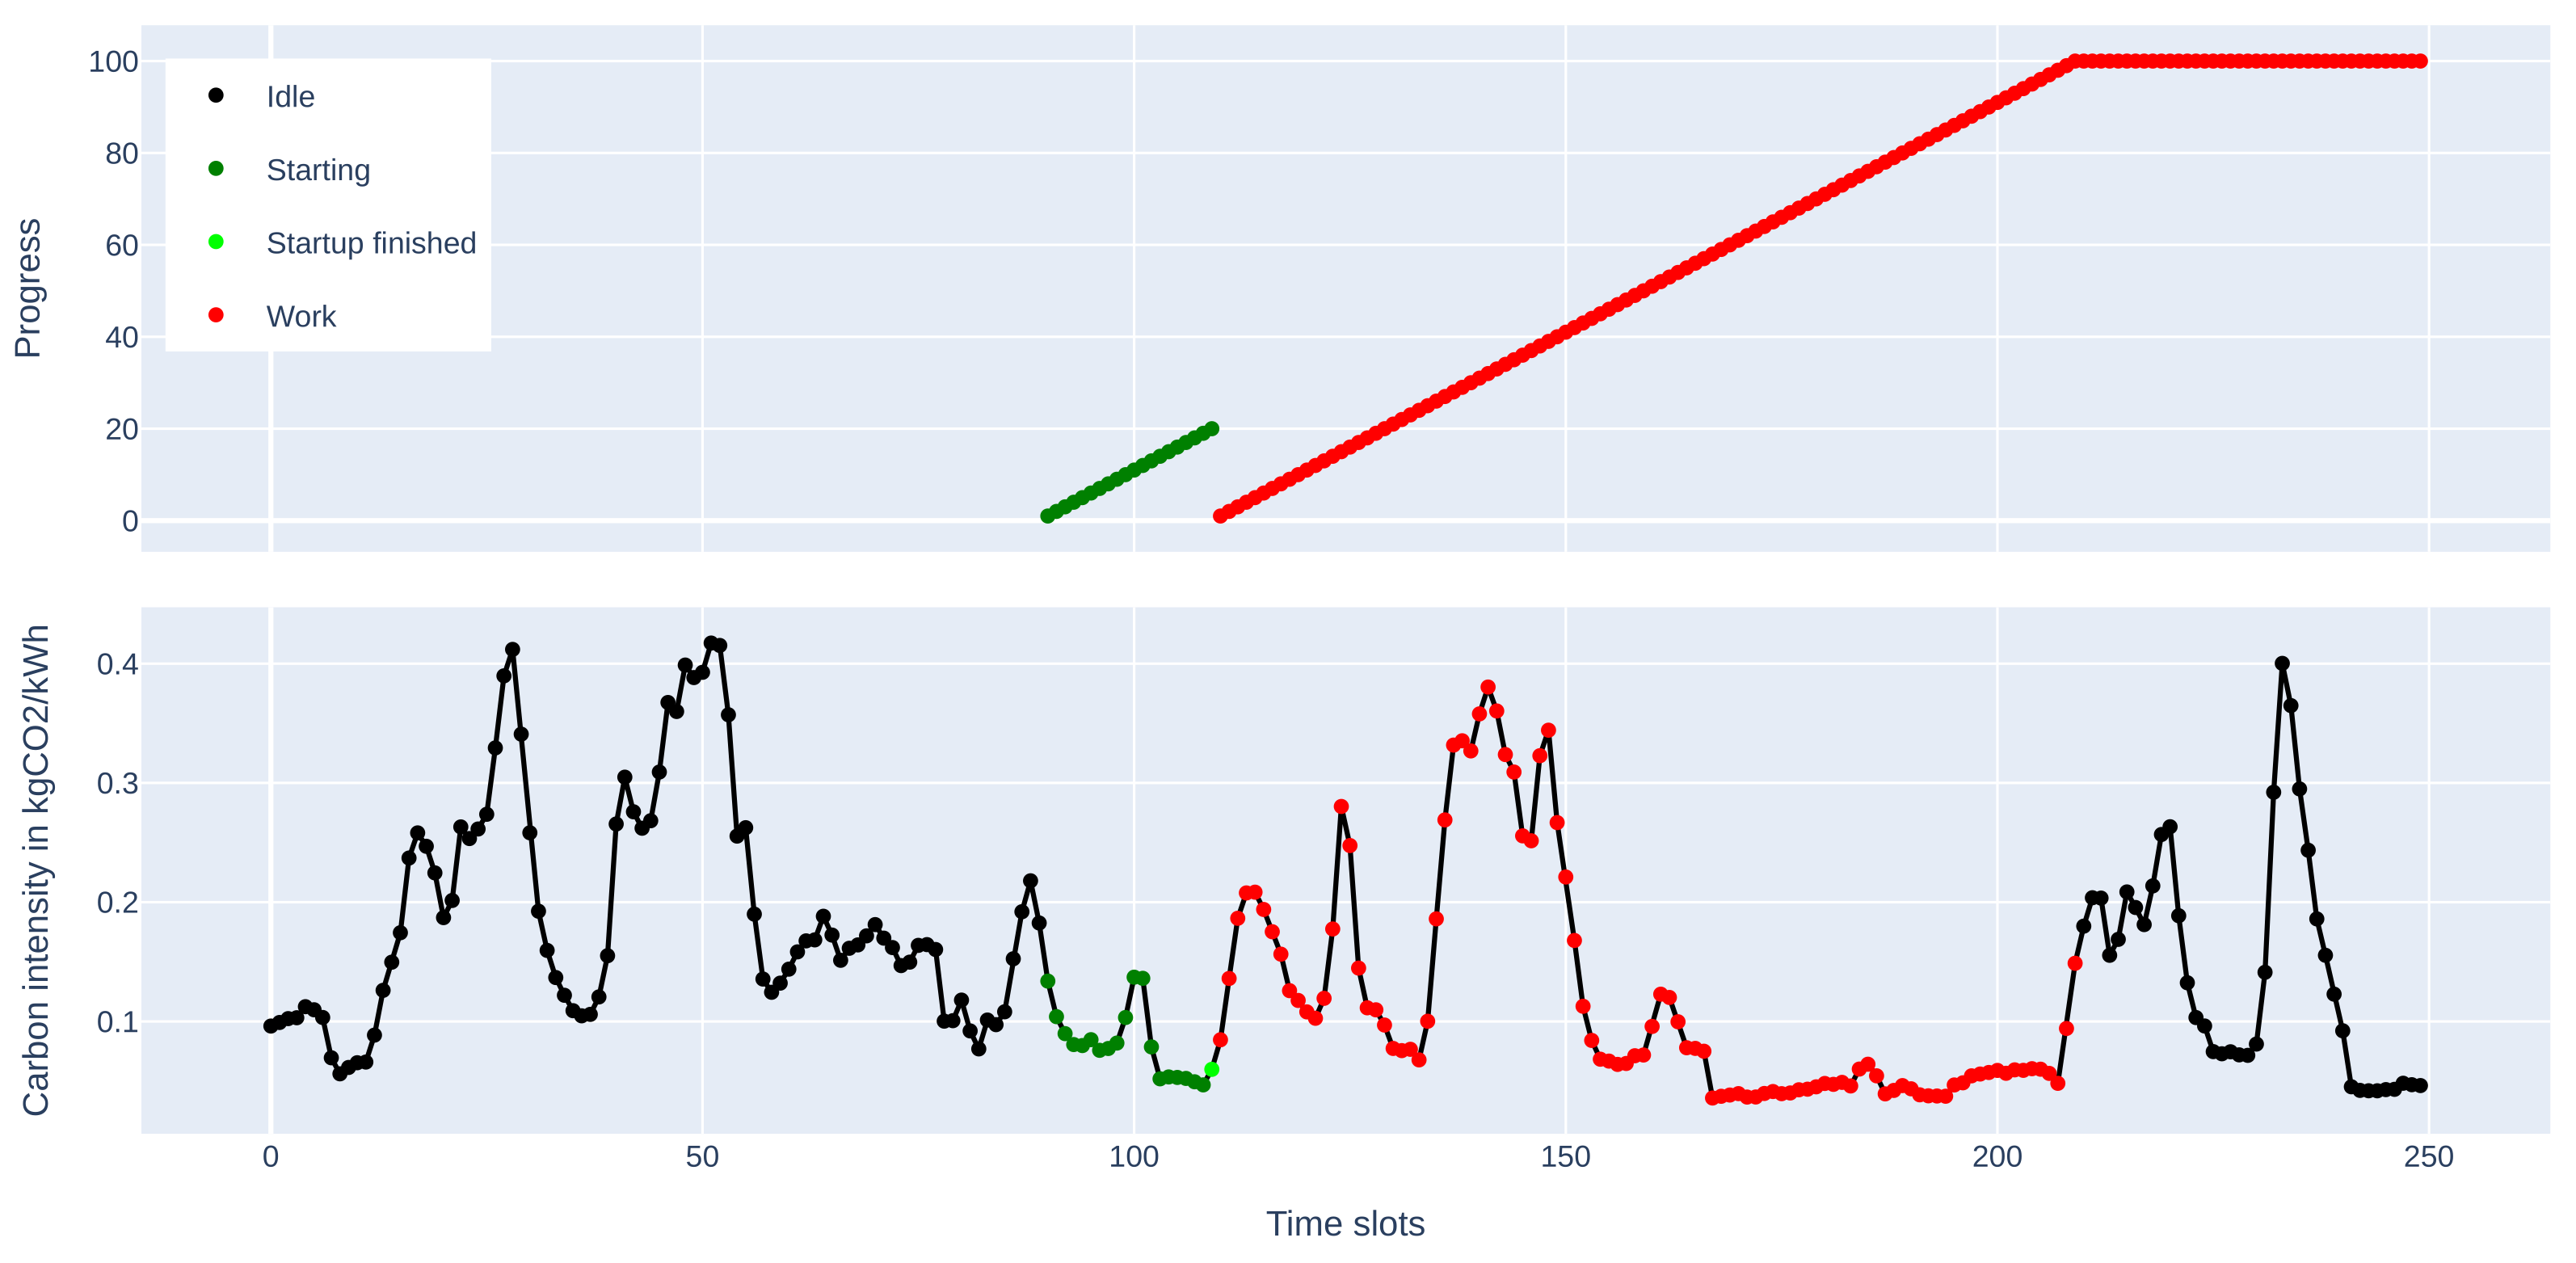
\includegraphics[width=\linewidth]{GAIA/notebooks/lp_progress.pdf}
    \caption{The result set now contains the progresses of the startup and work phase}
    \label{fig:lp_progress}
\end{figure}

\subparagraph{Adding dynamic power according to the new model}

The goal of this part will be to have an LP variable for each phase, which indicates when the job is in that phase.
When such indicators exist, the formula for calculating a schedule's carbon emissions can be changed to the following (\ref{formula:total_carbon}):

\begin{align}
    \label{formula:total_carbon}
    carbonEmitted(t) = \sum_{p \in Phases} isActive(p, t) * powerOfPhase(p) * carbonEmission(t)
\end{align}

With that goal in mind, we add the pseudocode listed in \ref{list:lp_phases} to determine when a phase is active. 

\begin{lstlisting}[frame=single, numbers=left, caption={Phase detection in LP}, label={list:lp_phases}, basicstyle=\ttfamily, breaklines]
# for each phase
# let phase_indicator, phase_indicator_upper, phase_indicator_lower be DEADLINE-many boolean variables

# set lower_bound to be the minimum progress this phase can occur in 
# set upper_bound to be the maximum similarly

# do the following for each phase
for t in range(DEADLINE):
    prob += progress[t] - lower_bound <= M*phase_indicator_lower[t]
    prob += lower_bound - progress[t] <= M*(1-phase_indicator_lower[t])

    prob += upper_bound - progress[t] <= M*phase_indicator_upper[t]
    prob += progress[t] - upper_bound <= M*(1-phase_indicator_upper[t])

    prob += phase_variable[t] >= phase_indicator_lower[t] + phase_indicator_upper[t] - 1
    prob += phase_variable[t] <= phase_indicator_lower[t]
    prob += phase_variable[t] <= phase_indicator_upper[t]
\end{lstlisting}

Unwrapping this, two helper variables are added per phase per time slot. 
A lower variable indicates that the previously established progress is above the threshold for a phase, while the upper variable indicates the opposite. 
The \verb|phase_variabel| is then "active" where these two overlap (line 14 to 17 define a logical "AND").

The constraint of line 8 is only applied if the indicator is \verb|false|.
If it is false, the progress at the time slot must be below the lower bound (as negative numbers are equal to 0).
Line 9 works on the negated indicator, applying the constraint if it is \verb|true|. 
If the indicator is \verb|true|, progress must be higher than the lower bound. 
Combining this, the expression \verb|phase_indicator_lower[t] <=> progress[t] > lower_bound| is added to the model. 
The upper bound is formulated in the following two lanes similarly.

Using this addition, the schedule now looks like the one shown in figure \ref{fig:lp_states}. 
Unlike the previous times, splitting the job up into two parts is now the optimal solution. 
Attention should be drawn to the circumstance that the high-powered phase (the green one) is scheduled on the lowest carbon emissions while the low-powered one is scheduled on the higher emission time slots.

\begin{figure}
    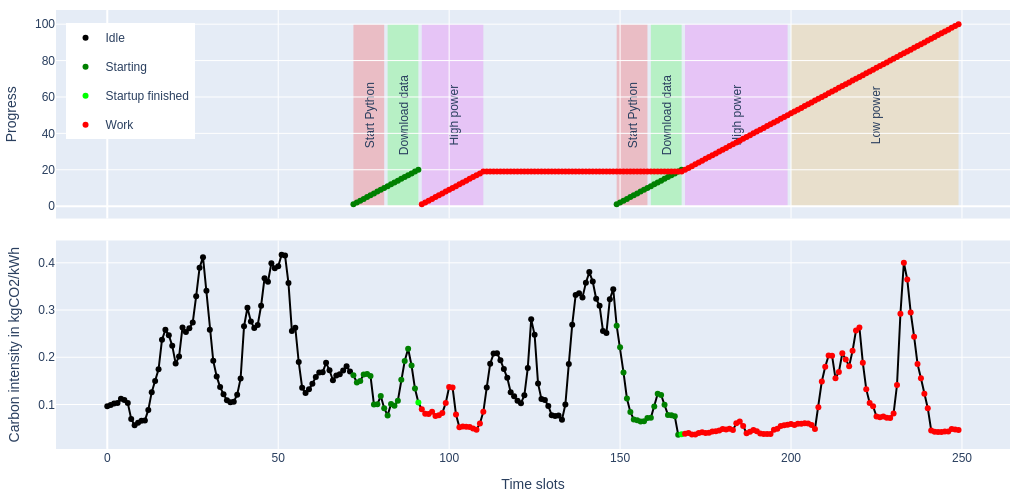
\includegraphics[width=\linewidth]{GAIA/notebooks/lp_states.pdf}
    \caption{The final scheduling including dynamic power via phases}
    \label{fig:lp_states}
\end{figure}

\subparagraph{Issues of the implementation}

As of now, checkpointing may happen at any point in the scheduler, as the \verb|work_progress| is never reset. 
Checkpointing at specific points, such as after specific phases like in the entry ML example in section, will be left for future work.\todo{Add this to future work!}

Another issue is the runtime and hardware requirements for finding a solution.
While the upper example of 250 time slots and a job length of 120 were found within minutes on my laptop (a Lenovo T470 with 8GB RAM and an i5-7200U CPU @ 2.50GHz), bigger problem sizes such as 5000 time slots and a length of 800 would barely finish within 30 minutes with a \emph{gap}-value of 98\%.
As the LP solver computes the problem, the gap value is an indicator of how close the solver is to finding the optimal solution, the optimal solution is found when the gap is at 0\%.

Solvers are able to take advantage of multiple CPU cores, but in my case, the issue was probably a lack of memory. 
Glancing into the system monitor utility on Ubuntu would show that all 8 GB are in use and that swap space is being used a lot.

\subparagraph{Decreasing the Problem Size}

In the previously shown Figures, each carbon-emission data point would correspond to one time slot, which in turn corresponds to one unit of time in the job. 
Going by the resolution of the carbon-emissions, each data point describes the emissions for one hour. 
In the original \verb|GAIA| implementation, job lengths are given in seconds, however. 
The example workload used for measuring in Section \ref{sec:power_measurements} also showed that timescales in seconds are useful. 

Using a 1:1 mapping between those would result in 3600 (60s * 60) time slots for each hour, resulting in very large problem sizes in turn needing long execution times and high amounts of memory.

In order to improve on the issues mentioned above, the following optimization is made: by calculating the \emph{greatest common divisor (gcd)} between all phase durations and the time resolution of the carbon-emissions (3600), all durations can be scaled down by the \verb|gcd|. Each time slot in the model would then represent \verb|gcd|-many seconds.

The effect of this optimization heavily depends on the input phases. 
If there are very short phases, the \verb|gcd| would likewise be low and problem size would not be decreased much. 

\todo[inline]{I could perhaps do a tiny evaluation on runtime and hardware usage, doing a cute lil graph with x being problem time, z being job length, y being runtime / memory usage}
	\chapter{Evaluation} \label{sec:evaluate_scheduling}

\section{Parameter Description}

In order to evaluate the carbon savings made possible by the previously established dynamic power model, the following approach is proposed:
As the already existing job traces hold no information regarding the power or their phases, some test cases will be presented and used for the models.
In a rather explorative process, we use the following parameters and run the simulation on all possible permutations of them. 
This is done using the \verb|generate_evaluation_jobs.sh| script, the used parameters are listed in the following table:

\begin{table}[h!]
    \centering
    \begin{tabular}{|p{0.3\linewidth}|p{0.6\linewidth}|}
    \hline
        Parameter & Values \\ \hline
        Scheduling Strategy & suspend \& resume, non-interrupted \\ \hline
        Phases & alternating high- and low-powered phases, each either 30 or 60 minutes long \\ \hline
        Startup length & no startup, 5 minutes, 10 minutes, 30 minutes \\ \hline
        Startup power level & 100 W, 200 W \\ \hline
        Waiting time & 4 hours, 12 hours, 1 day, 2 days \\ \hline
        Job length & 1, 2, and 3 hours \\ \hline
        Carbon trace & Week from July 1. 2024 (see Figure \ref{fig:energy_mix}) \\ \hline
    \end{tabular}
    \caption{Overview of the parameters used for the evaluation}
    \label{tab:evaluation_parameters}
    \end{table}

Another dimension will be comparing these scenarios against having no information on phases, instead only having an averaged constant wattage of the otherwise existing phases.
The latter represents the previous \verb|GAIA| implementation, where jobs had a constant amount of power at all points in time.
Finding the LP solution will time-limited to 20 minutes and all jobs will be simulated to be submitted at the very first time in the trace.

\todo[inline]{This needs some better explanation, the phases don't really make too much sense, perhaps just go with the generic ML-job setup I introduced earlier}

\section{Running the Evaluation on a Cluster}

As previously discussed in Section \ref{sec:checkpoint_resume_lp}, calculating suspend \& resume scheduling tends to have high runtime and memory requirements. 
For that reason, the simulation was executed on the \emph{SCORE Lab}, short for \emph{scientific compute resources}, of HPI.

After requesting and gaining access, \verb|rsync| was used to transfer the simulation to the cluster. 
Slurm could then be used to schedule all experiments individually (that were generated using the mentioned \verb|generate_all_jobs.sh| script), which would parallelize the evaluation, leading to faster results.

One problem arose in the licensing of the used \emph{Gurobi} solver. 
Under our academic license, only 2 \emph{sessions} are allowed simultaneously.
A session is defined via the hostname of the executing machine, which is communicated to the solver's licensing servers live.
As such, scheduling each experiment by itself lead to many sessions being started, as Slurm distributes the jobs on the available nodes.
While there is some leeway in the amount of sessions, experiments crashed beyond the 5th instance as the solver did not start.

We work under this restriction by distributing the experiments across two workers (via a script called \verb|evalute_dynamic_power.sh|); as each experiment has an index, one worker executes the even numbered jobs and the other executes the odd ones. 
Using the even-odd strategy results in both workers having about the same amount of work.

The workers in this case are python docker containers that were created with the help SCORE Lab's online knowledge base.\webcite{web_knowledgebase}
The command for launching one example worker, in this case the one for even jobs, is given in Listing \ref{list:evaluation_slurm}.

\begin{minipage}{\linewidth}
\begin{lstlisting}[language=bash, frame=single, numbers=left, caption={Executing the Evaluation inside the SCORE Lab's Slurm environment}, label={list:evaluation_slurm}, basicstyle=\ttfamily]
    sbatch -A polze -p magic \
        --container-image=python \
        --container-name=test \
        --container-writable \
        --mem=128G \
        --cpus-per-task=128 \
        --time=24:0:0 \
        --output=slurmlogs/output_%j.txt \
        --error=slurmlogs/error_%j.txt \
        --constraint=ARCH:X86 \
        --container-mounts=/hpi/fs00/home/vincent.opitz:/home/vincent.opitz \
        --container-workdir=/home/vincent.opitz/master-thesis/GAIA \
        run_all_even_jobs.sh
        \end{lstlisting}    
\end{minipage}

Now the simulation can be run with 128 GB RAM as specified in line 5. 
The \verb|-p magic| parameter results in us using a compute node. 
Line 3, \verb|--container-writable|, means that the container will be reused if called again under the same name, this lets us conduct set up  (\verb|pip install|).
Restricting the nodes to be \verb|X86| nodes via line 10 is necessary as there are other architectures available in the cluster. 
Without this line, Slurm can schedule our jobs on nodes incompatible to the containers' pre-compiled Python binary, resulting in an error on start\webcite{web_scoreslack}.

\section{Results}

Running the evaluation took a combined, and very carbon aware, processing time of 3 days and 16 hours split across two instances.
In sum, 1200 jobs were simulated with differing parameters. 

\subsection{Effect of Suspend-Resume Scheduling}

In the introductory research questions, we surmised that the effects of suspend-resume scheduling may be lessened under a model that contains startup costs for resuming. 
In order to answer this, we first calculate the total carbon emissions for each job under different schedulers. The GAIA and \programname{} output includes multiple entries per job if they get paused, so they get aggregated into the total.

With this, we first run an ANOVA to determine the axis under which to explore the data. Table \ref{tab:scheduler_anova}, shows that the length and phases of a job impact carbon emissions significantly.
This is not unexpected, however, as these parameters increase the time and overall energy required to run the job, in turn also increasing overall carbon emissions.
Waiting times being very significant as well, is consistent with existing literature\cite{wiesner_lets_2021}.

\begin{table}[h!]
    \centering
    \begin{tabular}{|c|c|c|}
    \hline
        Parameter & p\_value & p\_value (rounded) \\ \hline
        Job length & $0.000000e+00$ & $0.00$ \\ \hline
        Waiting time &  $1.008635e-23$ & $0.00$ \\ \hline
        Phases &  $1.910669e-04$ & $0.00$ \\ \hline
        Scheduling Algorithm &  $1.827666e-01$ & $0.18$ \\ \hline
        Startup power level &  $6.641101e-01$ & $0.66$ \\ \hline
        Phases averaged or not &  $7.436032e-01$ & $0.74$ \\ \hline
        Startup length &  $9.885010e-01$ & $0.99$ \\ \hline
    \end{tabular}
    \caption{Results of the ANOVA for total carbon emissions per scheduler. The lower the p-value, the higher the impact on carbon emissions.}
\label{tab:scheduler_anova}
\end{table}

With these findings, we will visualize jobs grouped by their length and waiting time, as their p-values are effectively zero.
In Figure \ref{fig:eval_different_schedulers}, all simulated jobs are plotted with their respective total carbon emissions. Blue indicates that both schedulers, with suspend \& resume and the other without, had the same emissions (within 0.01g). If the emissions are not equal, red and green dots indicate the respective scheduler performance.
The remaining parameters are hashed into an integer, showing that they have little effect on the carbon emissions.

By eye, it can be observed that the carbon savings between the schedulers are consistently minimal for jobs of length up to atleast 8 hours and for all jobs with waiting times up to 6 hours.
There are however, exception to this: for example, 8-hour jobs with a waiting time of 2 days exhibit saving potential, but only for jobs with a startup time of less 30 minutes (these are hashed to around 20). This can also be observed for hours of 16 hours but only 6 hours of waiting time.

The bottom right sub-plot, showing the maximum waiting time and job-length, does not follow the column trend of increased savings with increased waiting times. In a few cases, the suspend \& resume scheduler performs \emph{worse}, as can be seen by green dots being above all other dots.
One explanation for this can be seen in Figure \ref{fig:timelimited_gantt}, showing the scheduling for different job lengths, with a startup time of 5 minutes, a waiting time of 4 days.
Checking the Slurm logs for the jobs highlighted in red shows that the LP scheduler stopped after hitting the time limit of 20 minutes, only finding a result that is within the constraints but not optimal.
The gap value introduced in Section \ref{sec:checkpoint_resume_lp}, for these jobs is 100\%.
In fact, counting the occurrences of \verb|"Time limit reached"| in the logs shows that out of all jobs, 209 timeouts occurred. 
Since half of the 1200 jobs are LP-scheduled, about a third of them did not find an optimal solution in time.
The cumulative distribution for the time limited solutions in Figure \ref{fig:ecdf_gap} shows a heavy skew towards bad solutions, if the time limit is not kept.

\begin{figure}
    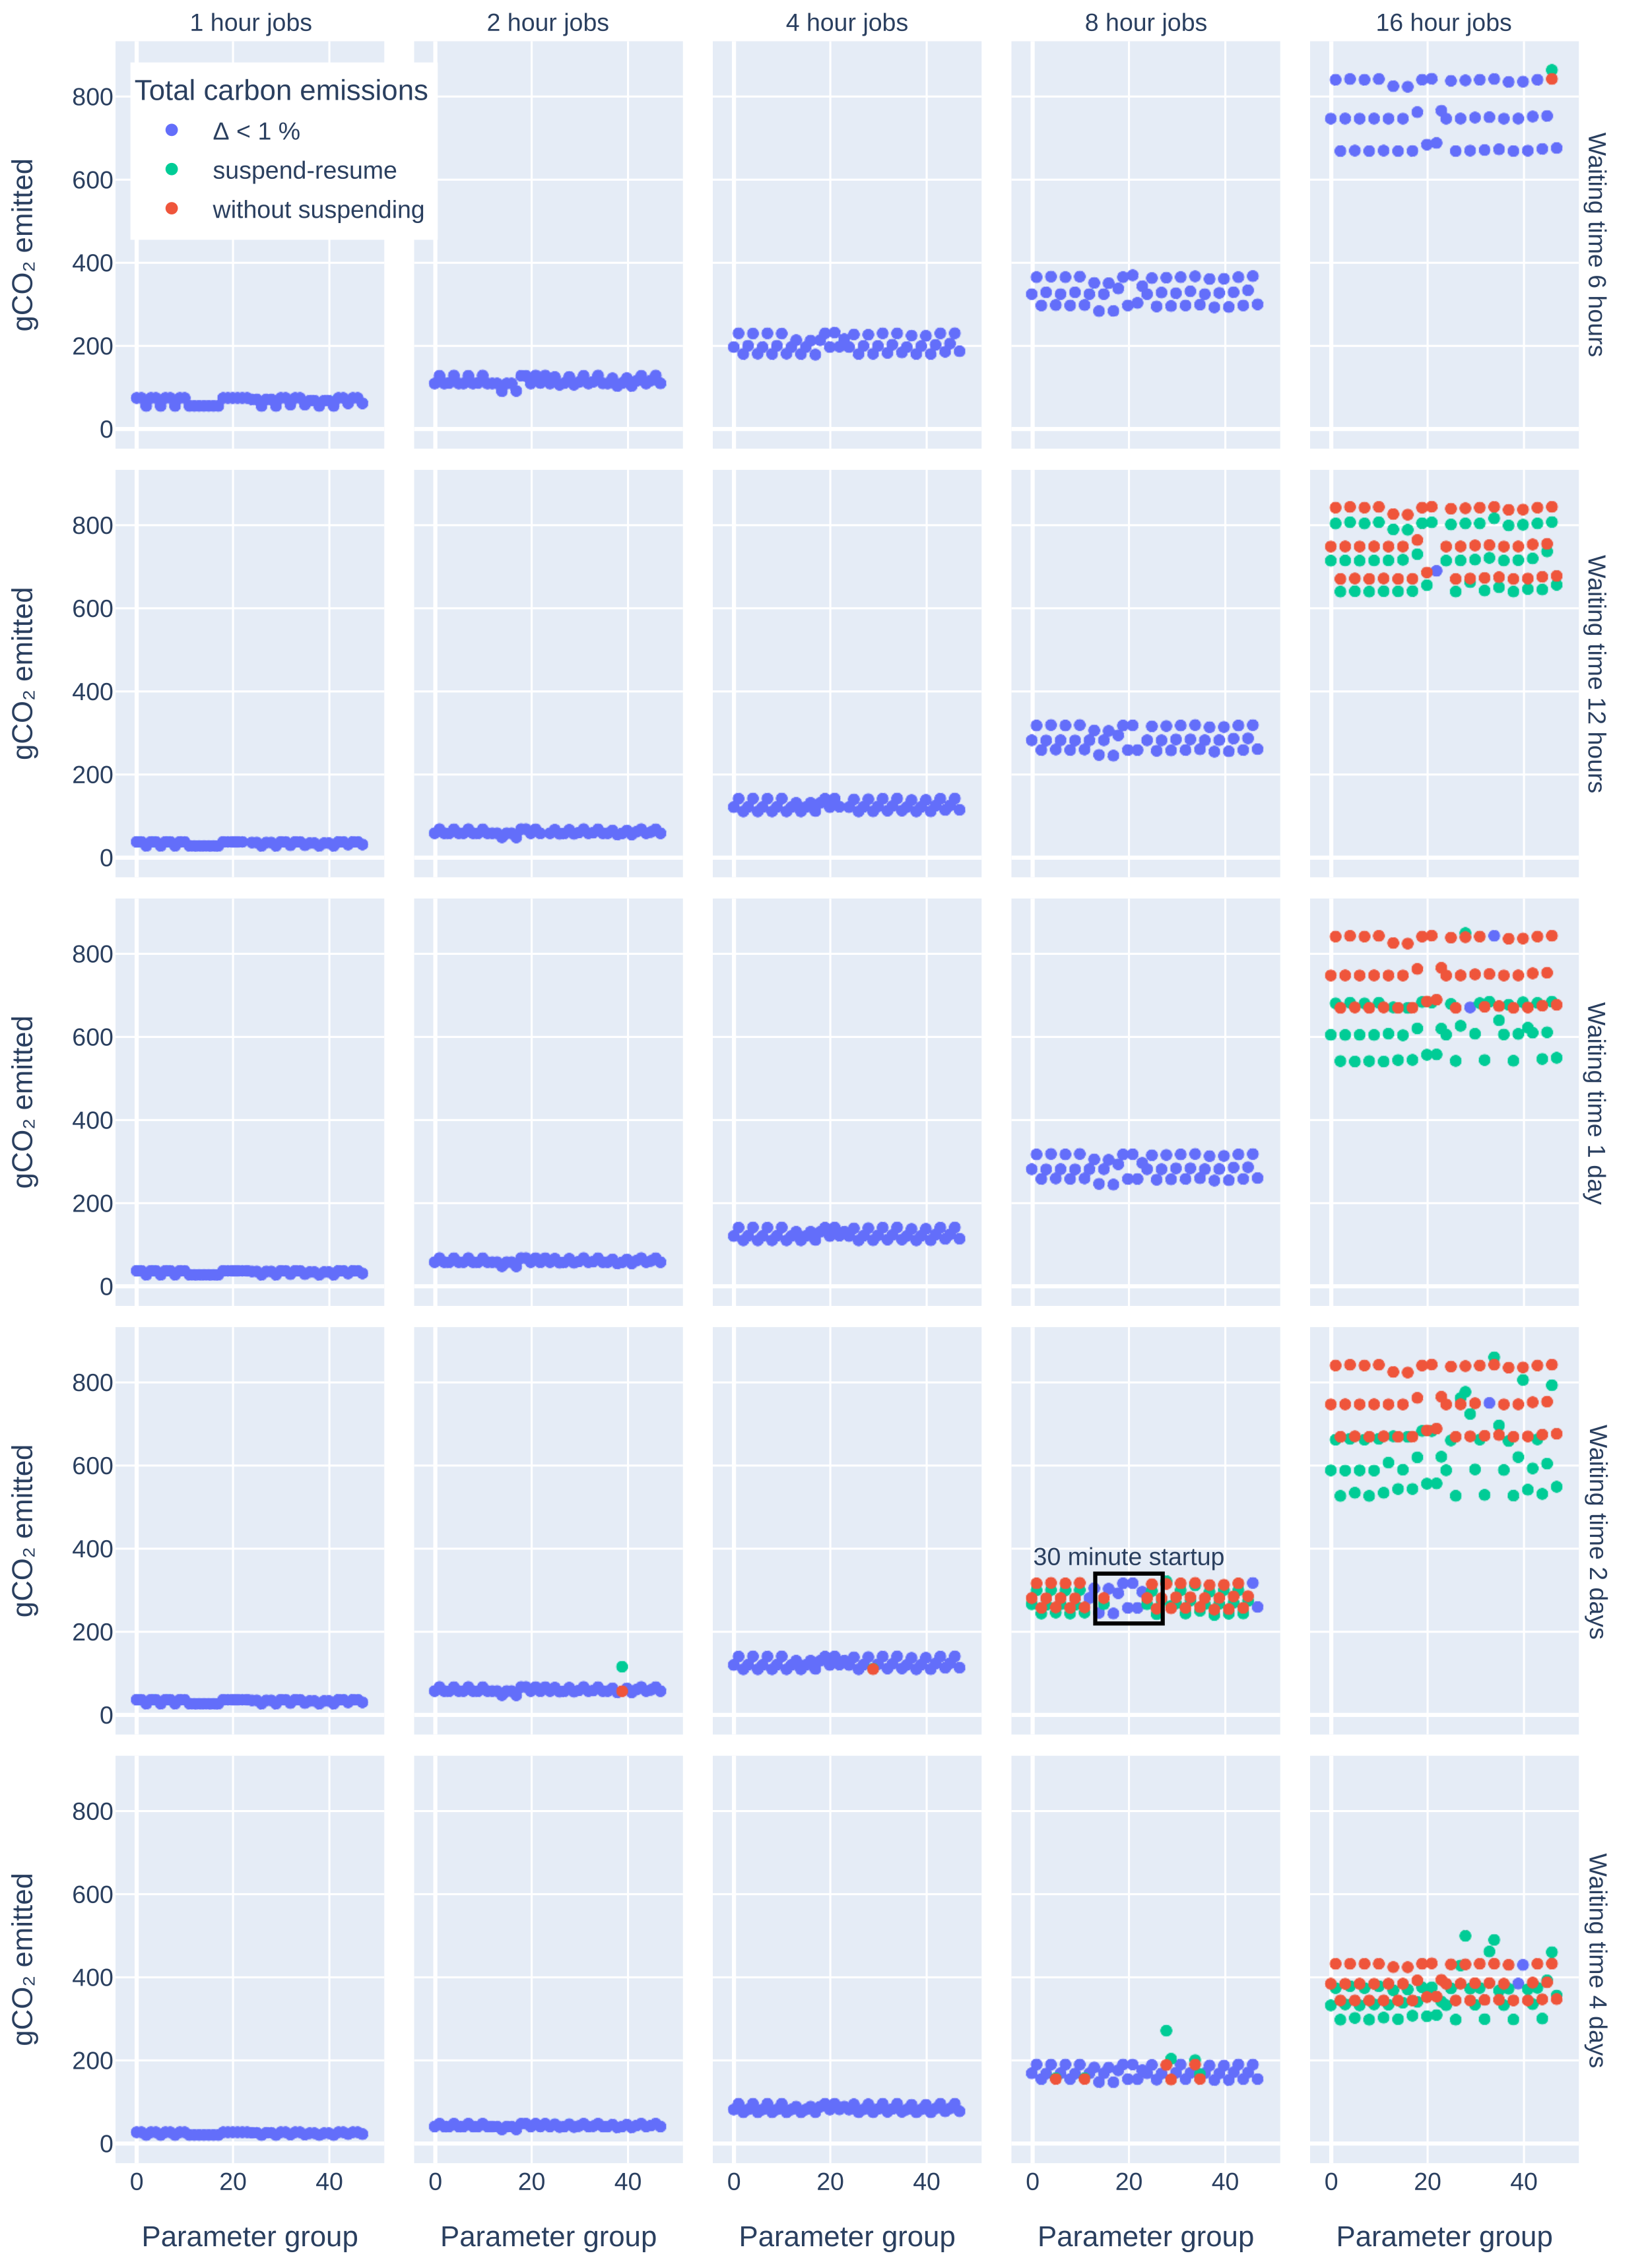
\includegraphics[width=\linewidth]{GAIA/notebooks/eval_same_job_different_schedulers.pdf}
    \caption[short]{All simulated jobs and their total carbon emissions, compared between the two scheduling approaches. Blue indicates equal emissions, red and green differentiate the schedulers. Each \emph{group} of jobs are different phases configurations.}
    \label{fig:eval_different_schedulers}
\end{figure}

\begin{figure}
    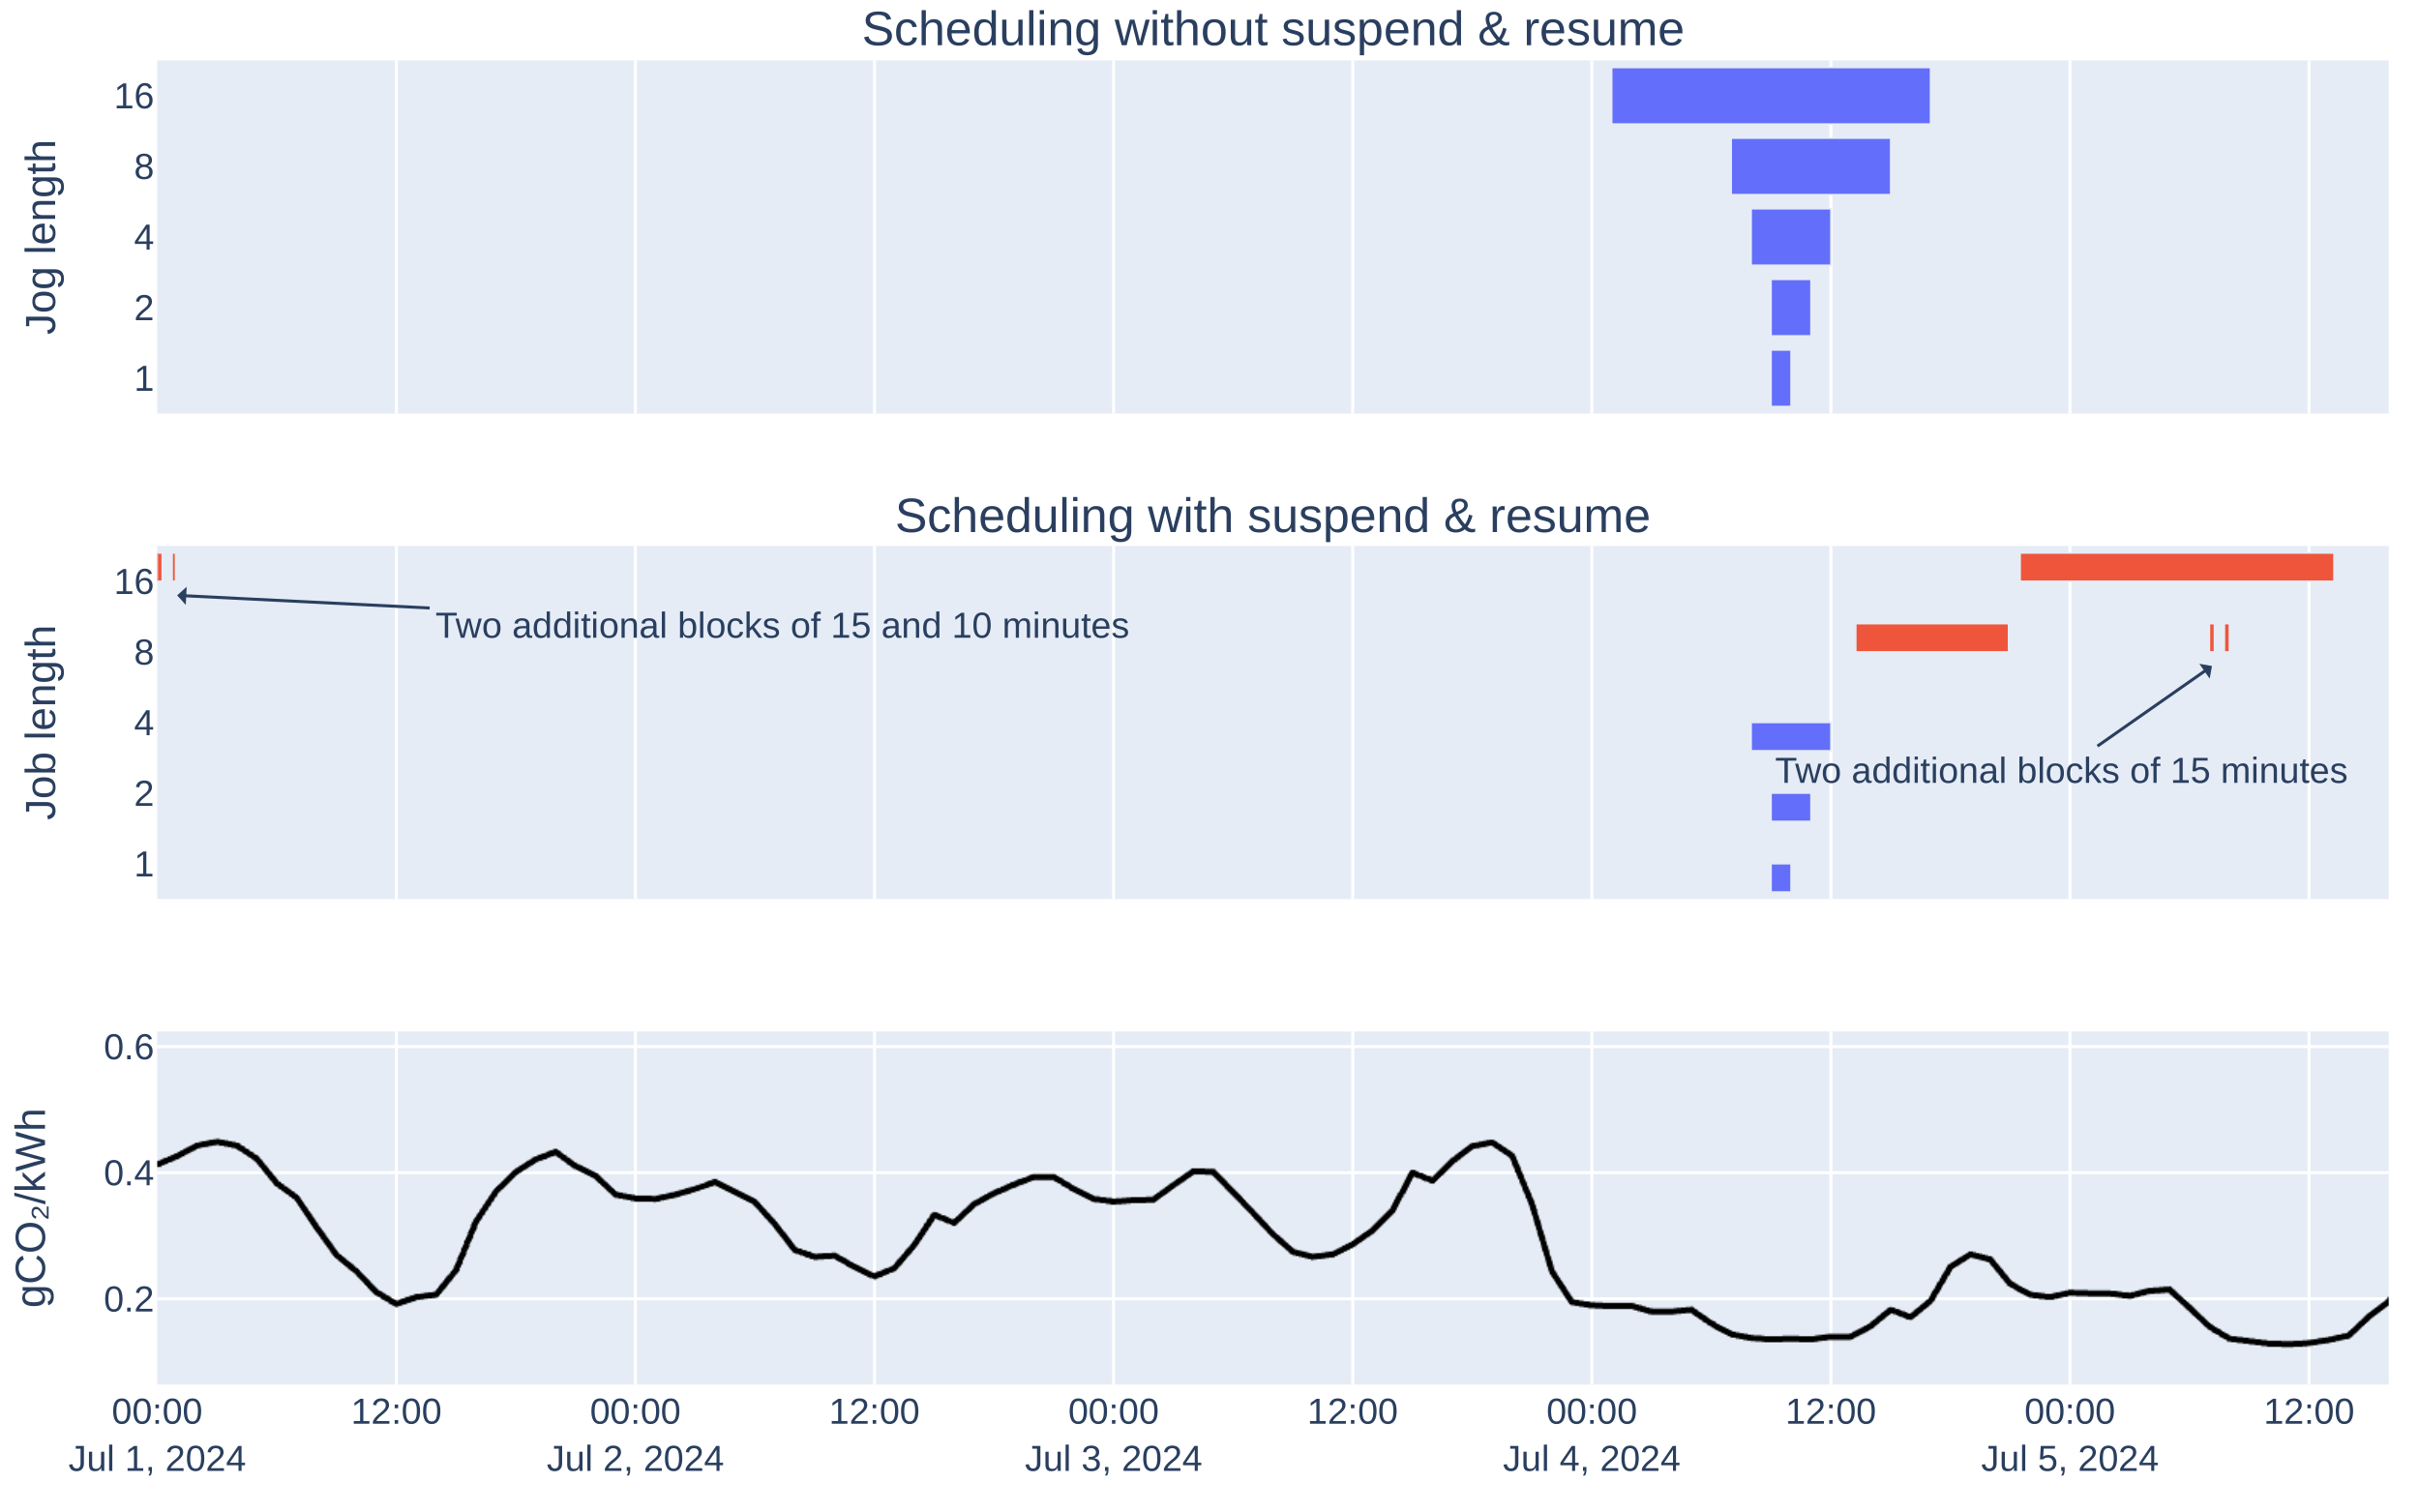
\includegraphics[width=\linewidth]{GAIA/notebooks/timelimited_gantt.pdf}
    \caption[short]{Schedules of jobs with different lengths under different schedulers. All Jobs have a waiting time of 4 days and a startup time of 5 minutes. The red bars suboptimal schedules that are found upon being time limited.}
    \label{fig:timelimited_gantt}
\end{figure}

\begin{figure}
    \includegraphics[width=\linewidth]{GAIA/slurmlogs/gap_value_ecdf.pdf}
    \caption[short]{Cumulative distribution plot of the gap value of time limited schedules. A higher gap indicates worse results. There is a heavy skew to 100\%, with half of the values being about 95\%}
    \label{fig:ecdf_gap}
\end{figure}

\section{Effect of Phases}


	\chapter{Results}

\begin{itemize}
    \item here we would try to show off the difference between power-and-phase-oblivious scheduling and my new implementation which can make use of that
    \item 
\end{itemize}
	\chapter{Discussion} \label{sec:discussion}

For this, we will discuss each contribution by itself and draw a conclusion in the end.

\section{\modelname{}}

With \modelname{}, we propose a high-level time-to-power model for workloads.hack around
In essence, it models a workload as having startup phases and work phases. 
Each of these then have a constant power attached to it. 
This presents a superset of the workload models used in prior literature in this field.
Using a constant per phase is a big simplification, however. 
The main motivation for this was to reduce complexity in the LP suspend \& resume scheduler.
We also argue that in the context of the low carbon-emission resolutions, this is appropriate.

A drawback of \modelname{} is that power used outside the job is not captured at all.
In a real-world cloud scenario, there will be e.g. be VM startup times \cite{zheng_benchmarking_2019}.
Also, we assume workloads to be executed in an isolated matter. 
Thus, each workload under \modelname{} increases power and carbon emissions linearly.
On real-world hardware however, servers have a baseline energy demand. 
Sharing resources and increasing utilization of a server increases energy efficiency \cite{barroso_case_2007}. 
Performance impacts due to shared hardware is also not part of \modelname{}.

In the context of long workloads and parallel execution, the clean-cut phases we observed on a single machine and a short job may 
not hold in HPC environments.

The effects of a baseline power in \modelname{} need further examination as well.
In our evaluation, we have decided not to exclude a baseline power. There, the startup costs where either 100 W or 300 W. As we observed for \verb|RoBERTa| in Section~\ref{sec:power_measurements}, the increase in power during startup was minimal. 
We argue that by using an unrestricted power-per-phase model, different use cases could be explored:
Including the baseline inside \modelname{} could be used to simulate settings where a machine would otherwise be turned off. 
Excluding the baseline could be used to simulate scheduling workloads on otherwise idling machines.


\section{\programname{}}

We iterated on an existing testbed, GAIA.
In comparison to prior work, workloads in \programname{} now have heterogeneous phases and their startup times are part of the scheduling.
We have tried to evaluate this changed assumption for different startup costs, different phases, waiting times, and job lengths. 
The trend that allowing resumeable jobs to be deferred for longer increases carbon savings \cite{wiesner_lets_2021,hanafy_going_2024, hanafy_war_2023}, appeared in our results as well. 
We were also able to observe the findings by Sukprasert et al. \cite{sukprasert_limitations_2024} that a suspend \& resume strategy benefits very long jobs more.

Wholly unexplored are the effects job heterogeneity that we added.
The reason being that our chosen scenarios:

\begin{itemize}
    \item Had phases of relatively short length. It is likely that longer phases result in more pronounced results.
    \item Used too many phases. We chose to repeat low and high phases until the given job length is met, meaning that the amount of phases increased linearly. As suspend \& resume scheduling works better for very long jobs, they could not be scheduled within a time limit of 20 minutes.
\end{itemize}

A drawback of the LP implementation is that computation time is dependent on the shortest phase in \modelname{} (see Section \ref{sec:checkpoint_resume_lp}). Thus, if startup times are short, they may need to be removed in favor of runtimes. The OPR approach described in Section \ref{sec:state_of_the_art}, which assumes startup to have a cost but no length, does not have this problem.

We want to propose a more fit approach to the evaluation:
First, a literature review of long-running workloads with long phases is necessary. Additionally, the power measurement capabilities of cluster nodes we described in Section \ref{sec:power_measurements} could be used to measure larger ML models than we were able to execute on our private hardware.
Given these workloads, the evaluation is then done under different carbon traces to remove bias.
In our evaluation, the days 4 and following had an influx of wind power which dominated the carbon savings for the longest waiting time. 

In our case, due to the way each job was generated and indexed, the hardest problems were executed last. 
A better approach would be to compute the complex problems first to check whether time limits are hit, or to run them in a random order.
Running a sample evaluation for select parameters should also have been done.
As of now, the impact of our used parameters on the resulting LP complexity is not entirely clear.
A runtime analysis on \programname{}' LP scheduler could be a guide on what can be scheduled.

\section{Future Work} \label{sec:future_work}

There are several avenues for future work.
Regarding \programname{}, our suspend \& resume implementation is not yet able to make use of \modelname{}'s checkpoint annotations. Future work includes evaluating carbon-aware scheduling when jobs can only be checkpoint at some points.

Our LP scheduler showed long runtimes for more complex scheduling problems.
Future work could deal with either improving model performance \webcite{web_gurobi_threads,web_gurobi_optimization} or evaluating whether a break-even point in scheduling-time and carbon-saving exists.

We found that suspend \& resume scheduling works best for long jobs.
Future work could investigate which real-world workloads exhibit power heterogeneity.
Their saving potential our workload model could then be analyzed.

Instead of only testing predefined workloads, our LP scheduler could be combined with current research in the field of workload analysis. 
Köhler et al. \cite{kohler_recognizing_2021} classify workloads based on power signatures. 
On live systems, such an approach could be used to opt-in to a suspend \& resume strategy. 
We found that short jobs exhibit little potential carbon savings. 
If a workload then runs longer, classifying them as suspendible could lead to hybrid scheduling strategies.  

\section{Conclusion}

In our work, we conducted a structured literature review to outline state-of-the-art work on carbon-aware scheduling.
By conducting power measurements on a machine learning workload, we highlighted shortcomings in the workload model that is used in prior work and inferred our own model.
Namely, we proposed \modelname{}. 
It includes startup and work phases with differing power levels.
We then showcased how \modelname{} can be used in our testbed \programname for two distinct carbon-aware schedulers:
one simulated the execution of non-suspendible workloads and the other uses linear programming for suspend \& resume scheduling.
We evaluated the effect of \modelname{} against the state-of-the-art model throughout different parameters.
We found that, prior findings, such as increased carbon savings through longer workload deadlines in suspend \& resume scheduling, still hold under \modelname{} even under different startup costs.
The effects of workload phases on carbon emissions will be part of future work. 
However, with \programname{}, such research can be conducted.
	\chapter{Future Work}



	% Bibliographie
	\ifisbook\cleardoubleemptypage\fi
	\phantomsection\addcontentsline{toc}{chapter}{\refname}
	\printbibliography[heading=subbibliography, title={Literature}, category={cited}, notkeyword={web}]
	\printbibliography[heading=subbibliography, title={Web Sources}, category={cited}, keyword={web}]
	

	% ggf. Anhang
	%\appendix\appendix
\thispagestyle{plain} % Yes, I just did that. ඞ
\section{Repository}
\section{Results of the Structured Literature Review}
 % example

	% ggf. bei englischen Arbeiten den deutschen Abstract nach hinten verschieben
	% \ifisbook\pagestyle{plain}\cleardoubleemptypage\include{content/abstract_deu}\fi

	% Eigenständigkeitserklärung
	\ifisbook\pagestyle{plain}\cleardoubleemptypage% => Laut Aussage des Studienreferats braucht es - auch wenn die Arbeit in englischer Sprache verfasst ist - KEINE separate Version der Eigenständigkeitserklärung auf Englisch. Sowohl für Arbeiten in deutscher Sprache als auch für Arbeiten in englischer Sprache genügt EINE EINZIGE Eigenständigkeitserklärung auf DEUTSCH.
\begin{otherlanguage}{ngerman}

\begin{center}\textsf{\textbf{Eidesstattliche Erklärung}}\end{center}
Hiermit versichere ich, dass meine {\thesistype} mit dem Titel \enquote{\thesistitle} (\enquote{\thesistitleother}) selbständig verfasst wurde und dass keine anderen Quellen und Hilfsmittel als die angegebenen benutzt wurden. Diese Aussage trifft auch für alle Implementierungen und Dokumentationen im Rahmen dieses Projektes zu.\\

\noindent
Potsdam, den \thesishandindate
\vspace{2cm}

\begin{center}
\begin{tabular}{C{6cm}}
\hline
{\small({\thesisauthor})}
\end{tabular}
\end{center}

\end{otherlanguage}\fi

\end{document}